%%%%%%%% ICML 2025 EXAMPLE LATEX SUBMISSION FILE %%%%%%%%%%%%%%%%%

\documentclass{article}

% Recommended, but optional, packages for figures and better typesetting:
\usepackage{microtype}
\usepackage{graphicx}
\usepackage{booktabs} % for professional tables
\usepackage{makecell}
\usepackage{pifont}
\usepackage{xcolor}

\usepackage{graphicx}
\usepackage{booktabs}
\usepackage{subcaption}

\usepackage[percent]{overpic}
\usepackage{hyperref}

\newcommand{\graycell}[1]{\cellcolor{gray!20}#1}

\usepackage{tikz}
\usepackage{pgfplots}
\usetikzlibrary{decorations.markings}
\pgfplotsset{compat=newest}
%%%%%%%%%%%%%%%%%%%%%%%%%%%%%%%%

\usepackage{tikz}
\usepackage{pgfplots}
\pgfplotsset{compat=newest}
\usetikzlibrary{shapes}

\usepackage{tikz}
\usetikzlibrary{shapes.symbols}
\usepackage{pgfplots}
\pgfplotsset{compat=newest}
\usepackage{xcolor}
\usepackage{pifont}
\usepackage{makecell}
\usepackage{booktabs}
\pgfplotsset{compat=1.18}
\usepackage{multirow}
\usepackage{colortbl}
\usetikzlibrary{fadings}
%----------------------------------------------------------------
% Core Marker Definitions (one definition per model)
% Each macro accepts a mandatory coordinate argument and an optional scale parameter.
% The coordinate argument MUST be given in parentheses.
%----------------------------------------------------------------

% 1) EfficientViT: Circle marker (default scale assumed 1.0)
\definecolor{myEfficientColor}{HTML}{D900CD}
\newcommand{\efficientColor}{myEfficientColor}
\DeclareRobustCommand{\EfficientMarker}[2][1.0]{%
  \filldraw[\efficientColor, scale=#1] #2 +(-2pt,-2pt) rectangle ++(4pt,4pt);%
}

% 2) SHViT: Square marker
\definecolor{myShvitColor}{HTML}{010000}
\newcommand{\shvitColor}{myShvitColor}
\DeclareRobustCommand{\ShvitMarker}[2][1.0]{%
  \filldraw[\shvitColor, rotate around={45:#2}, scale=#1] #2 +(-2pt,-2pt) rectangle ++(4pt,4pt);%
}


% 3) MobileNetV4: Triangle marker
\definecolor{myMobileColor}{HTML}{00D90D}
\newcommand{\mobileColor}{myMobileColor}
\DeclareRobustCommand{\MobileMarker}[2][1.0]{%
  \filldraw[\mobileColor, scale=#1] #2 ++(0pt,2pt) -- ++(-2pt,-4pt) -- ++(4pt,0pt) -- cycle;%
}

% 4) ViT+Registers: Star marker
% We allow an optional scale parameter; default scale for plots is 1.0.
\definecolor{myRegisterColor}{HTML}{D97900}
\newcommand{\registerColor}{myRegisterColor}
\DeclareRobustCommand{\RegisterMarker}[2][1.0]{%
    \filldraw[\registerColor, scale=#1] #2 circle (3pt);%
}

% 5) ViT+Jumbo
\definecolor{myJumboColor}{HTML}{0060D9}
\newcommand{\jumboColor}{myJumboColor}
\DeclareRobustCommand{\JumboMarker}[2][1.0]{%
  \node[
    shape=star,
    star points=5,
    star point ratio=2.25,
    draw=\jumboColor,
    fill=\jumboColor,
    scale=#1
  ] at #2 {};%
}
% \definecolor{myJumboColor}{HTML}{6129D6}
% \newcommand{\jumboColor}{myJumboColor}
% \DeclareRobustCommand{\JumboMarker}[2][1.0]{%
%   \filldraw[\jumboColor, rotate around={45:#2}, scale=#1] #2 +(-2pt,-2pt) rectangle ++(4pt,4pt);%
% }

%----------------------------------------------------------------
% Inline Marker Macros for Moving Arguments (e.g., tables)
% These call the above core macros with no argument (thus defaulting to (0,0))
% and specify a small scale (here 0.3) so the marker appears small in text.
%----------------------------------------------------------------
\newcommand{\InlineEfficientMarker}{%
  \mbox{\tikz[baseline=-0.6ex]{\EfficientMarker[0.6]{(0,0)}}}%
}
\newcommand{\InlineShvitMarker}{%
  \mbox{\tikz[baseline=-0.6ex]{\ShvitMarker[0.6]{(0,0)}}}%
}
\newcommand{\InlineMobileMarker}{%
  \mbox{\tikz[baseline=-0.6ex]{\MobileMarker[1.0]{(0,0)}}}%
}
\newcommand{\InlineRegisterMarker}{%
  \mbox{\tikz[baseline=-0.6ex]{\RegisterMarker[0.8]{(0,0)}}}%
}
\newcommand{\InlineJumboMarker}{%
  \mbox{\tikz[baseline=-0.6ex]{\JumboMarker[0.4]{(0,0)}}}%
}

% hyperref makes hyperlinks in the resulting PDF.
% If your build breaks (sometimes temporarily if a hyperlink spans a page)
% please comment out the following usepackage line and replace
% \usepackage{icml2025} with \usepackage[nohyperref]{icml2025} above.
\usepackage{hyperref}


% Attempt to make hyperref and algorithmic work together better:
\newcommand{\theHalgorithm}{\arabic{algorithm}}

% Use the following line for the initial blind version submitted for review:
% \usepackage{icml2025}

% If accepted, instead use the following line for the camera-ready submission:
\usepackage[accepted]{icml2025}

% For theorems and such
\usepackage{amsmath}
\usepackage{amssymb}
\usepackage{mathtools}
\usepackage{amsthm}
\definecolor{jumbo_color}{HTML}{9335CA}

\newcommand{\circlednum}[2][black]{\strut\raisebox{-1pt}{\tikz{\node[circle,inner sep=0.6pt,fill=#1,font=\scriptsize\bfseries\color{white}]{#2};}}}
\newcommand\SmallCaption[1]{%
  \captionsetup{font=scriptsize}%
  \caption{#1}}

% if you use cleveref..
\usepackage[capitalize,noabbrev]{cleveref}

%%%%%%%%%%%%%%%%%%%%%%%%%%%%%%%%
% THEOREMS
%%%%%%%%%%%%%%%%%%%%%%%%%%%%%%%%
\theoremstyle{plain}
\newtheorem{theorem}{Theorem}[section]
\newtheorem{proposition}[theorem]{Proposition}
\newtheorem{lemma}[theorem]{Lemma}
\newtheorem{corollary}[theorem]{Corollary}
\theoremstyle{definition}
\newtheorem{definition}[theorem]{Definition}
\newtheorem{assumption}[theorem]{Assumption}
\theoremstyle{remark}
\newtheorem{remark}[theorem]{Remark}

% Todonotes is useful during development; simply uncomment the next line
%    and comment out the line below the next line to turn off comments
%\usepackage[disable,textsize=tiny]{todonotes}
\usepackage[textsize=tiny]{todonotes}


% The \icmltitle you define below is probably too long as a header.
% Therefore, a short form for the running title is supplied here:
\icmltitlerunning{Simpler Fast Vision Transformers with a Jumbo CLS Token}

\begin{document}

\twocolumn[
\icmltitle{Simpler Fast Vision Transformers with a Jumbo CLS Token}

% It is OKAY to include author information, even for blind
% submissions: the style file will automatically remove it for you
% unless you've provided the [accepted] option to the icml2025
% package.

% List of affiliations: The first argument should be a (short)
% identifier you will use later to specify author affiliations
% Academic affiliations should list Department, University, City, Region, Country
% Industry affiliations should list Company, City, Region, Country

% You can specify symbols, otherwise they are numbered in order.
% Ideally, you should not use this facility. Affiliations will be numbered
% in order of appearance and this is the preferred way.
% \icmlsetsymbol{equal}{*}

\begin{icmlauthorlist}
\icmlauthor{Anthony Fuller}{car}
\icmlauthor{Yousef Yassin}{car}
\icmlauthor{Daniel G. Kyrollos}{car}
\icmlauthor{Evan Shelhamer}{ubc,vec}
\icmlauthor{James R. Green}{car}
\end{icmlauthorlist}

\icmlaffiliation{car}{Carleton University, Ottawa, Canada.}
\icmlaffiliation{ubc}{University of British Columbia, Vancouver, Canada.}
\icmlaffiliation{vec}{Vector Institute}

\icmlcorrespondingauthor{Anthony Fuller}{anthonyfuller@cmail.carleton.ca}

% You may provide any keywords that you
% find helpful for describing your paper; these are used to populate
% the "keywords" metadata in the PDF but will not be shown in the document
\icmlkeywords{Machine Learning, ICML}

\vskip 0.3in
]

% this must go after the closing bracket ] following \twocolumn[ ...

% This command actually creates the footnote in the first column
% listing the affiliations and the copyright notice.
% The command takes one argument, which is text to display at the start of the footnote.
% The \icmlEqualContribution command is standard text for equal contribution.
% Remove it (just {}) if you do not need this facility.

\printAffiliationsAndNotice{}  % leave blank if no need to mention equal contribution
% \printAffiliationsAndNotice{\icmlEqualContribution} % otherwise use the standard text.

\begin{abstract}

We introduce a simple enhancement to the global processing of vision transformers (ViTs) to improve accuracy while maintaining throughput.
Our approach, Jumbo, creates a wider \texttt{CLS} token, which is split to match the patch token width before attention, processed with self-attention, and reassembled.
After attention, Jumbo applies a dedicated, wider FFN to this token.
Jumbo \emph{significantly} improves over ViT+Registers \cite{darcet2024vision} on ImageNet-1K at high speeds (by $3.2\%$ for ViT-tiny and $13.5\%$ for ViT-nano); these Jumbo models even outperform specialized compute-efficient models while preserving the architectural advantages of plain ViTs.
Although Jumbo sees no gains for ViT-small on ImageNet-1K, it gains $3.4\%$ on ImageNet-21K over ViT+Registers.
Both findings indicate that Jumbo is most helpful when the ViT is otherwise too narrow for the task.
Finally, we show that Jumbo can be easily adapted to excel on data beyond images, e.g., time series.

\end{abstract}

\section{Introduction}
\label{submission}

\begin{figure*}
    \centering
    \includegraphics[width=\textwidth]{imgs/corel_arc.pdf}
    \caption{Overview of \gls{method}. Past residuals are used as input to a hybrid global-local graph-based quantile network.}
    \label{fig:corel}
\end{figure*}

There has been tremendous progress in computer vision over the past decade. Innovations have resulted in models with greater absolute accuracy, greater speed for a given accuracy, and greater simplicity. Vision transformers (ViTs) \cite{dosovitskiy2021an} exemplify this progress.

ViTs are \emph{simple}.
They split an image into patches, linearly project patches to form patch embeddings, add position embeddings to patch embeddings, prepend a learnable ``\texttt{CLS}'' token, and then process this set of vectors with a transformer; these operations can be implemented in a single file of ${\sim}100$ lines of PyTorch \cite{paszke2019pytorch} \footnote{For example: \url{https://github.com/lucidrains/vit-pytorch/blob/main/vit_pytorch/vit.py}}.
ViTs are \emph{flexible}.
They offer seamless sparse computation via token dropping \cite{he2022masked, akbari2021vatt, liu2023patchdropout}, patch resizing \cite{beyer2023flexivit, liu2024mspe}, image size extrapolating \cite{fuller2024lookhere}, model scaling \cite{zhai2022scaling, dehghani2023scaling}, and multimodal processing \cite{dou2022empirical, xu2023multimodal}.
ViTs are \emph{effective}.
They achieve state-of-the-art (SOTA) performance in image classification \cite{touvron2022deit, alabdulmohsin2024getting}, object detection \cite{li2022exploring, liu2025grounding}, and semantic segmentation \cite{li2024transformer}; ViTs are core components of vision-language models \cite{Qwen-VL, liu2023llava}.
However, plain ViTs often underperform more specialized architectures w.r.t. compute efficiency, especially at high speeds.

% a bit more concise
Many recent architectures improve the computational efficiency of ViTs \cite{cai2023efficientvit, mehta2021mobilevit, vasufastvit2023, yun2024shvit}, where an improvement in efficiency typically refers to achieving a better accuracy-speed trade-off.
These architectures leverage a \emph{hierarchical} design, following classic architectures, such as ResNets \cite{he2016deep} and VGGNets \cite{simonyan2014very} --- they progressively reduce spatial dimensions while increasing channel width.
A larger width corresponds to a larger feedforward network (FFN), which increases model capacity by enabling non-linear processing over more dimensions.
Yet, the \emph{cost} of larger FFNs is controlled in these architectures by decreasing the number of patches/tokens.
We highlight this added capacity at little computational cost as a common element of such models.
These efficient architectures typically intersperse modules such as convolutions, pooling, sparse or linear attention, and other innovations with standard ViT modules (i.e., self-attention and point-wise FFNs).
However, these innovations eliminate the desirable properties of plain ViTs we wish to keep, such as token dropping and multimodal support.

Increasing the depth and/or width is the standard approach to increase ViT model capacity \cite{zhai2022scaling}.
Recently \citet{darcet2024vision} increase the number of parameters by adding learnable tokens called ``registers''.
% learnable input tokens, called ``registers''.
Registers scale capacity asymmetrically by adding global capacity (= inter-token modeling) without adding local capacity (intra-token modeling).
This addresses a key weakness in ViTs that they identify: \emph{plain ViTs have insufficient global capacity}.
They show that adding registers improves the classification and segmentation performance of plain ViTs.
However, the global information in registers only interacts through attention (i.e., a weighted sum of linear projections).
This limits the ability of ViT+Registers to learn more complex functions of global features, which we address here.

Our method, called Jumbo, increases the width of the \texttt{CLS} token to $J$ times the patch width.
Before self-attention, our method splits this extra wide Jumbo token into $J$ smaller tokens, includes them in self-attention, and then concatenates them to reassemble a single Jumbo token.
Rather than sharing FFN parameters with all patches, Jumbo leverages a wider \texttt{CLS}-specific FFN to increase model capacity.
The cost of this larger FFN is minimal because it only processes a single token.
Crucially, Jumbo preserves all the advantages of plain ViTs previously discussed, while efficiently adding global capacity.
This includes support for token dropping, which is critical for many self-supervised learning (SSL) algorithms \cite{wei2025towards, assran2023self, he2022masked, fu2024rethinking}. 

We show that ViT+Jumbo significantly outperforms ViT+Registers in three scenarios through apples-to-apples comparisons.
Specifically, Jumbo clearly improves in image classification: \circlednum{1} on ImageNet-1k at ViT-tiny and ViT-nano sizes, and \circlednum{2} on ImageNet-\emph{21k} at sizes up to ViT-base.
These results lead to an insight: Jumbo is helps most when the ViT is otherwise too narrow for the task.

In fact, ViT+Jumbo at tiny and nano scales outperforms specialized compute-efficient architectures, such as EfficientViT \cite{cai2023efficientvit}.
To our knowledge, ViT+Jumbo is the first attention-only and non-hierarchical architecture to even be competitive with compute-efficient architectures at high speeds.
These two properties make ViT+Jumbo compatible out-of-the-box with SOTA SSL and adaptable to other data modalities such as time series.

\circlednum{3} As an example of applying Jumbo beyond vision, we show that the simple incorporation of Jumbo for time series tasks improves performance over PatchTST \cite{Yuqietal-2023-PatchTST} and PatchTST+Registers.

\section{Background and Related Work}

\subsection{Vision Transformers}

A ViT splits an image into a grid of non-overlapping patches, $\mathbb{R}^{Y \times X \times C}\to \mathbb{R}^{N_y \times N_x \times P_y \times P_x \times C}$, where $C$ is the number of channels, $Y$ / $X$ are the image height / width, $N_y$ / $N_x$ are the grid height / width, and $P_y$ / $P_x$ are the patch height / width in pixels (equal to $\frac{Y}{N_y}$ / $\frac{X}{N_x}$). Next, they flatten the grid into a sequence and flatten the patches into vectors, $\mathbb{R}^{N_y \times N_x \times P_y \times P_x \times C}\to \mathbb{R}^{N \times D_{pix}}$, where $N$ is the number of patches (equal to $N_y \cdot N_x$), and $D_{pix}$ is the number of pixel values per patch (equal to $P_y \cdot P_x \cdot C$). Next, they apply a learnable linear projection to form patch embeddings, $\mathbb{R}^{N \times D_{pix}}\to \mathbb{R}^{N \times D}$, where $D$ is the model width, also known as the embedding dimension. Next, they add position embeddings to patch embeddings. (Superior and slightly more complex position encoding methods exist \cite{weinzaepfel2023croco, heo2025rotary, fuller2024lookhere}; however, we simply use learnable embeddings in this work --- although Jumbo is also compatible with all these other methods.) These operations produce local tokens $\mathbf{x}^{P}\in \mathbb{R}^{N \times D}$ that represent \emph{highly} local information --- typically a $16\times16$ px square. Crucially for this work, ViTs prepend a learnable \texttt{CLS} token $\mathbf{x}^{\texttt{CLS}}$ to the sequence of local tokens, $\mathbf{x} = \mathbf{x}^{\texttt{CLS}} \Vert_{0} \mathbf{x}^{P} \in \mathbb{R}^{(N+1) \times D}$, where $\Vert_{0}$ denotes concatenation along the $0^{\text{th}}$ (sequence) dimension. Finally, the input $\mathbf{x}$ is processed by a plain transformer and the --- now contextualized --- \texttt{CLS} token can be used for image classification.

\textbf{Sizes.} ViT sizes vary w.r.t. depth and width. The models we train all have $12$ layers, while the widths vary $\{96, ~128, ~192, ~384, ~768\}$, corresponding to names $\{$pico$, ~$nano$, ~$tiny$, ~$small$, ~$base$\}$. We name pico and nano sizes inspired by \citet{woo2023convnext}.

A standard image size of $224\times224$ px and a standard patch size of $16\times16$ px results in $196$ local tokens. A \emph{single} \texttt{CLS} token --- that is designed to aggregate global information to facilitate classification --- provisions $1/197^{\text{th}}$ of a model's representational capacity to global information (and this fraction decreases with larger images and/or smaller patches). This allocation seems suboptimal. Recent work finds evidence to support this intuition and proposes a fix.

\textbf{Registers.} \citet{darcet2024vision} find that ViTs are so hungry for more \texttt{CLS} tokens that they \emph{learn} to repurpose some local patch tokens into ``pseudo-\texttt{CLS}'' tokens; these co-opted tokens behave like \texttt{CLS} tokens --- they aggregate global information and discard patch-specific local information. \citet{darcet2024vision} propose a fix: prepend additional learnable tokens --- called registers $\mathbf{x}^{\texttt{Reg}}\in\mathbb{R}^{R \times D}$, where $R$ is the number of registers --- to the input sequence, $\mathbf{x} = \mathbf{x}^{\texttt{CLS}} \Vert_{0} \mathbf{x}^{\texttt{Reg}} \Vert_{0} \mathbf{x}^{P} \in \mathbb{R}^{(N+R+1) \times D}$. Registers improve performance and reduce attention map artifacts by provisioning more global capacity. 

Adding registers is elegantly simple to implement, and they preserve the advantages of plain ViTs; they can natively drop tokens and are compatible with SOTA self-supervised learning algorithms. In theory, registers can benefit any plain, noncausal transformer. These several advantages account for registers' \emph{significant and immediate} impact, including their application beyond image data \cite{dong2024hymbahybridheadarchitecturesmall, vaquero2024lost, leigh2024tokenization, messaoud2025towards, hu2024fm, thimonier2024t, omranpour2024higher}. For these reasons, ViT+Registers is the primary inspiration behind our method, Jumbo.

\textbf{Hiera.} Our work aligns spiritually with Hiera \cite{ryali2023hiera}, simplifying hierarchical transformers, such as Swin \cite{liu2021swin} or MViT \cite{fan2021multiscale}, by replacing convolutions with pooling layers. Although hierarchical models are incompatible with token dropping out-of-the-box, \citet{ryali2023hiera} engineer a solution allowing Hiera to be pretrained with masked autoencoding \cite{he2022masked}. However, Hiera is not fast --- e.g., its fastest variant has $0.58 \times$ the throughput of our Jumbo ViT-small.

\subsection{Compute Efficient Architectures}\label{sec:compute-efficient}

We highlight $3$ architectures and use them as baselines for a high-speed ViT. \circlednum{1} EfficientViT \cite{cai2023efficientvit} and \circlednum{2} SHViT \cite{yun2024shvit} improve the efficiency of ViTs by incorporating efficient attention, pooling, and convolutional layers. \circlednum{3} MobileNetV4 \cite{qin2025mobilenetv4} improves the efficiency of CNNs by leveraging many strategies (and different strategies for different model sizes). These baselines represent the SOTA in computational efficiency; please refer to Appendix \ref{appendix:related_work} for descriptions of these model architectures.

\definecolor{orangeFFN}{HTML}{D79B00}
\definecolor{blueFFN}{HTML}{0060D9}

\begin{figure*}
\centering
\begin{tikzpicture}[font=\sffamily]
	\node (image) at (0,0) {
        \includegraphics[width=\textwidth]{sophia.pdf}
	};
    \node[
      anchor=west,
      label={[yshift=0.8cm, xshift=-8.6cm]above:{\bfseries ViT+Jumbo (ours)}}, % Text on top
      text width=0.46\textwidth,
      align=center,
      minimum height=3cm
    ] (left) at (0,0) {};

    \node[
      anchor=west,
      label={[yshift=0.8cm, xshift=0.24cm]above:{\bfseries ViT+Registers \cite{darcet2024vision}}}, % Text on top
      text width=0.46\textwidth,
      align=center,
      minimum height=3cm
    ] (left) at (0,0) {};
\end{tikzpicture}
\vspace{-0.75cm}
\caption{
\textbf{(Left)} Our ViT+Jumbo method creates a wider \texttt{CLS} token that gets split into several tokens, with width equal to the patch width, prior to multi-headed self-attention (MHSA). After attention, the split Jumbo \texttt{CLS} token is reassembled via concatenation, and is then processed by {\textbf{\color{blueFFN}{\emph{its own} FFN}}}. Patches are processed by {\textbf{\color{orangeFFN}{their own, shared FFN}}}. \textbf{(Right)} ViT+Registers creates many register tokens all equal to the patch width. All registers, patches, and the \texttt{CLS} token are processed by {\textbf{\color{orangeFFN}{a shared FFN}}}. ViT+Jumbo enhances global processing as the (split) global tokens can interact via an FFN, in addition to attention.
}\label{fig:sophia}
\end{figure*}  


Beyond these, there is a rich literature on compute-efficient computer vision architectures. For example, several efficient CNN-based architectures exist \cite{howard2017mobilenets, sandler2018mobilenetv2, howard2019searching, han2020ghostnet, tan2019mnasnet, vasu2023mobileone}; however, these have been recently surpassed by MobileNetV4 \cite{qin2025mobilenetv4}. Since the invention of the ViT \cite{dosovitskiy2021an}, there have been many compute-efficient ``ViTs'' that incorporate efficient modules inspired by CNN-based approaches \cite{vasufastvit2023, mehta2021mobilevit, mehta2022separable, li2023rethinking, pan2022edgevits, chen2022mobile, li2022efficientformer}. SHViT \cite{yun2024shvit} has recently surpassed these architectures. Despite their impact and ingenuity, none of these hybrid architectures meets the definition of a plain ViT, which is attention-only and non-hierarchical; they thus lose many advantages of ViTs that we wish to keep.

\section{Method}

\subsection{Design Motivation and Intuition}
\textbf{Capacity.} Registers increase the global capacity of plain ViTs. Registers ``communicate'' with each other through attention. And attention is best thought of as a mechanism that \emph{moves} information between tokens \cite{elhage2021mathematical}. While the attention sublayer is a crucial component of transformers, its expressive capacity, alone, is inherently limited. Conversely, an FFN (equivalent to an MLP with $1$ hidden layer) accepts a single token as input, and processes this information by applying a learned non-linear function. By concatenating our global tokens (i.e., the split Jumbo token) and sending the resultant Jumbo token through an FFN, we can model more complex functions of global features.

\begin{table}[t]
\begin{minipage}{1.0\linewidth}
\begin{sc}
% \begin{flushright}
\caption{FLOPs breakdown of Group-MATES processes.}
\vspace{-0.2cm}
\label{tab:breakdown}
\vskip 0.15in
\resizebox{1.0\linewidth}{!}{%
\begin{tabular}{lrr}
\toprule
\textbf{Process} & \textbf{\#FLOPs $*$1e19} & \textbf{Ratio} \\
\midrule 
\multicolumn{2}{l}{\textbf{400M-4x Setting:} 412M model, 32.8B tokens}\\
\midrule
Model pretraining & 8.00 & 87.8\% \\
Oracle data influence collection & 0.29 & 3.2\% \\
Data influence model training & 0.01 & 0.1\% \\
Bootstrapping data influence model & 0.04 & 0.4\% \\
Data influence model inference & 0.77 & 8.5\% \\
\textbf{Total} & {9.11} & {100\%} \\
\midrule
\multicolumn{2}{l}{\textbf{1B-1x Setting:} 1.4B model, 28.0B tokens}\\
\midrule
Model pretraining & 24.00 & 93.3\% \\
Oracle data influence collection & 1.01 & 3.9\% \\
Data influence model training & 0.01 & 0.1\% \\
Bootstrapping data influence model & 0.04 & 0.2\% \\
Data influence model inference & 0.65 & 2.5\% \\
\textbf{Total} & {25.71} & {100\%} \\
\bottomrule
\end{tabular}
}
\end{sc}
% \end{flushright}
\end{minipage}
\vspace{-0.5cm}
\end{table}

\textbf{Cost.} Although Jumbo adds global capacity, its cost is minimal. The key insight is that the larger FFNs only process a single token. As shown in Fig. \ref{fig:flops}, the primary drivers of computational cost (FLOPs per layer) are sequence length and patch width, $D$. The FLOP contribution from adding registers or our Jumbo token is comparatively negligible. We discuss Jumbo's parameter increase in Section \ref{sec:discussion}.

\textbf{Non-hierarchical and attention-only.} Jumbo preserves the non-hierarchical (sometimes called columnar or isotropic) shape of ViTs and ViT+Registers. And, by foregoing convolutions, spatial information only moves through attention. These features have several advantages that we now discuss.

\circlednum{1} Attention-only models can efficiently \textbf{drop tokens}. Although convolutions are capable of processing a sparse subset of patches via sparse compute kernels, these kernels can be complex, challenging to use, and require updating when new hardware arrives. Furthermore, sparse convolutional kernels will never be as efficient as simply indexing from a sequence --- i.e., how transformers drop tokens. As one point of comparison, ConvNeXt V2 \cite{woo2023convnext} reports a $1.3\times$ speedup using a $60\%$ masking ratio with the Minkowski Engine v0.5.4 \cite{choy20194d}. Conversely, MAE \cite{he2022masked} report $2.8-4.1\times$ speedups using a $75\%$ masking ratio with plain ViTs. Efficient token dropping is required for most SOTA SSL algorithms, for example, I-JEPA \cite{assran2023self}, CrossMAE \cite{fu2024rethinking}, Image World Models \cite{garrido2024learning}, LatentMIM \cite{wei2025towards}, etc. Token dropping is also used to speedup plain supervised training \cite{dehghani2024patch}; we demonstrate this use of token dropping in subsection \ref{subsec:21k}. 

\circlednum{2} Non-hierarchical and attention-only models can be easily adapted to \textbf{other data modalities}. For example, $1$D time series, $3$D point clouds, or multimodal data; users need only adjust tokenization strategies. We demonstrate a $1$D time series application of Jumbo in subsection \ref{subsec:time}. 

\circlednum{3} Non-hierarchical and attention-only models can more easily benefit from other deep learning advances; i.e., they can \textbf{``piggyback'' off other innovations}. \circlednum{a} Many recent SSL methods are designed for the plain ViT's non-hierarchical shape \cite{wei2025towards, assran2023self, garrido2024learning}. \circlednum{b} Many recent segmentation and object detection ``heads'' are designed for the plain ViT's non-hierarchical shape \cite{fang2023unleashing, liu2025grounding, zhang2022segvit}. \circlednum{c} Many recent advances in compute kernels for plain self-attention decrease its cost. For example, Flash Attention \cite{dao2022flashattention, dao2023flashattention, shah2024flashattention} can speed up self-attention by more than $5\times$. Jumbo immediately benefits from these advances.

Conversely, \emph{none} of the compute-efficient architectures cited in subsection \ref{sec:compute-efficient} immediately benefit from these advances. None of them support other data modalities. And none of them support token dropping.

\textbf{Two hypotheses.}
Jumbo asymmetrically increases the network width.
Thus, \circlednum{1} we expect increasing gains due to Jumbo with \emph{decreasing} patch token width.
In other words, the more width-deprived a network, the more Jumbo should help.
However, what it means to be ``width-deprived'' is not straightforward.
Intuitively, tasks requiring reasoning over \emph{more concepts} must require \emph{more width} to store these concepts and facilitate reasoning over them.
Thus, \circlednum{2} we expect increasing gains due to Jumbo with \emph{increasing} task output dimensionality.
We explore both of these hypotheses using experiments with ViTs of different widths and datasets of different complexities.

\subsection{Design Specifics}

Exactly like the original ViT, Jumbo computes patch embeddings, $\mathbf{x}^{P}\in\mathbb{R}^{N \times D}$. Unlike the original ViT, our method creates a Jumbo \texttt{CLS} token that is $J$ times wider than the patch width $D$, $\mathbf{x}^{\texttt{Jumbo}}\in\mathbb{R}^{J \cdot D}$. Architecturally identical transformer layers then process these inputs.

Before self-attention, the Jumbo token is split into $J$ tokens, $\mid^{1}_{J}\mathbf{x}^{\texttt{Jumbo}} : \mathbb{R}^{1 \times J \cdot D} \rightarrow \mathbb{R}^{J \times D}$, where $\mid^{1}_{J}$ denotes splitting into $J$ segments along the $1^{\text{st}}$ (feature) dimension. Next, the split Jumbo token is concatenated with patch embeddings along the sequence dimension, $\mathbf{x} = \mathbf{x}^{\texttt{Jumbo}} \Vert_{0} \mathbf{x}^{P} \in \mathbb{R}^{(N+J) \times D}$. This sequence is sent through a plain multi-headed self-attention layer. Afterward, the Jumbo token is extracted from the sequence by splitting along the sequence dimension, $\mid^{0}_{2}\mathbf{x} : \mathbb{R}^{(N+J) \times D} \rightarrow (\mathbb{R}^{J \times D}, \mathbb{R}^{N \times D})$, where the first element contains the (still split) Jumbo token and the second element contains the patch representations. Finally, the Jumbo token is reassembled through concatenation along the channel dimension, $\mathbf{x}^{\texttt{Jumbo}} = \Vert_{1} \mathbf{x}^{\texttt{Jumbo}} : \mathbb{R}^{J \times D} \rightarrow \mathbb{R}^{1 \times J \cdot D}$. These two splits and two concatenations add negligible runtime overhead.

After self-attention, the Jumbo token is processed by its own FFN; i.e., it does not share parameters with the patch-wise FFN. We indicate this in Fig. \ref{fig:sophia} by coloring Jumbo and patch-wise FFNs differently. After all layers process the image, our method projects the Jumbo token to $C$ class logits, $\mathbb{R}^{J \cdot D} \rightarrow \mathbb{R}^{C}$. Since the patch-wise FFNs in the last layer are unused, we discard them.

\section{Experiments}

For all experiments, we measure throughput on an RTX 4090 GPU using PyTorch 2.6.0, \texttt{torch.compile}, and a $512$ batch size. 

\subsection{High-Speed Experiments}\label{subsec:1k}

We take a different experimental approach to many prior works. Typically, these works train models with their novel architecture on ImageNet-1K for $300$ epochs. They perform (often extensive) tuning and directly compare with results reported by baselines. For example, MobileNetV4 \cite{qin2025mobilenetv4} tunes the architecture for each model scale (small, medium, etc.) using neural architecture search (NAS). Furthermore, each model scale is often trained with a different hyperparameter ``recipe'' --- in the case of MobileNetV4 each recipe comprises $10+$ hyperparameters that seem tuned. This methodology results in \emph{highly} valuable artifacts --- i.e., trained model weights --- that practitioners can download and use.

However, this approach makes building atop such research challenging, as the relative contributions between architecture and training recipe can be unclear. Furthermore, the robustness of the results w.r.t. the training recipe can also be unclear, leading to significant uncertainty when leveraging the novel architecture in different settings. 

Informed by these observations, we perform apples-to-apples comparisons, which includes training SOTA high-speed models ourselves.

\begin{figure*}[ht!]
\begin{minipage}{0.99\textwidth}
    \centering
    %-------------------------------------------------
    % First row of plots
    %-------------------------------------------------
    \hspace{-0.6cm}
    \begin{subfigure}[b]{0.22\textwidth}
        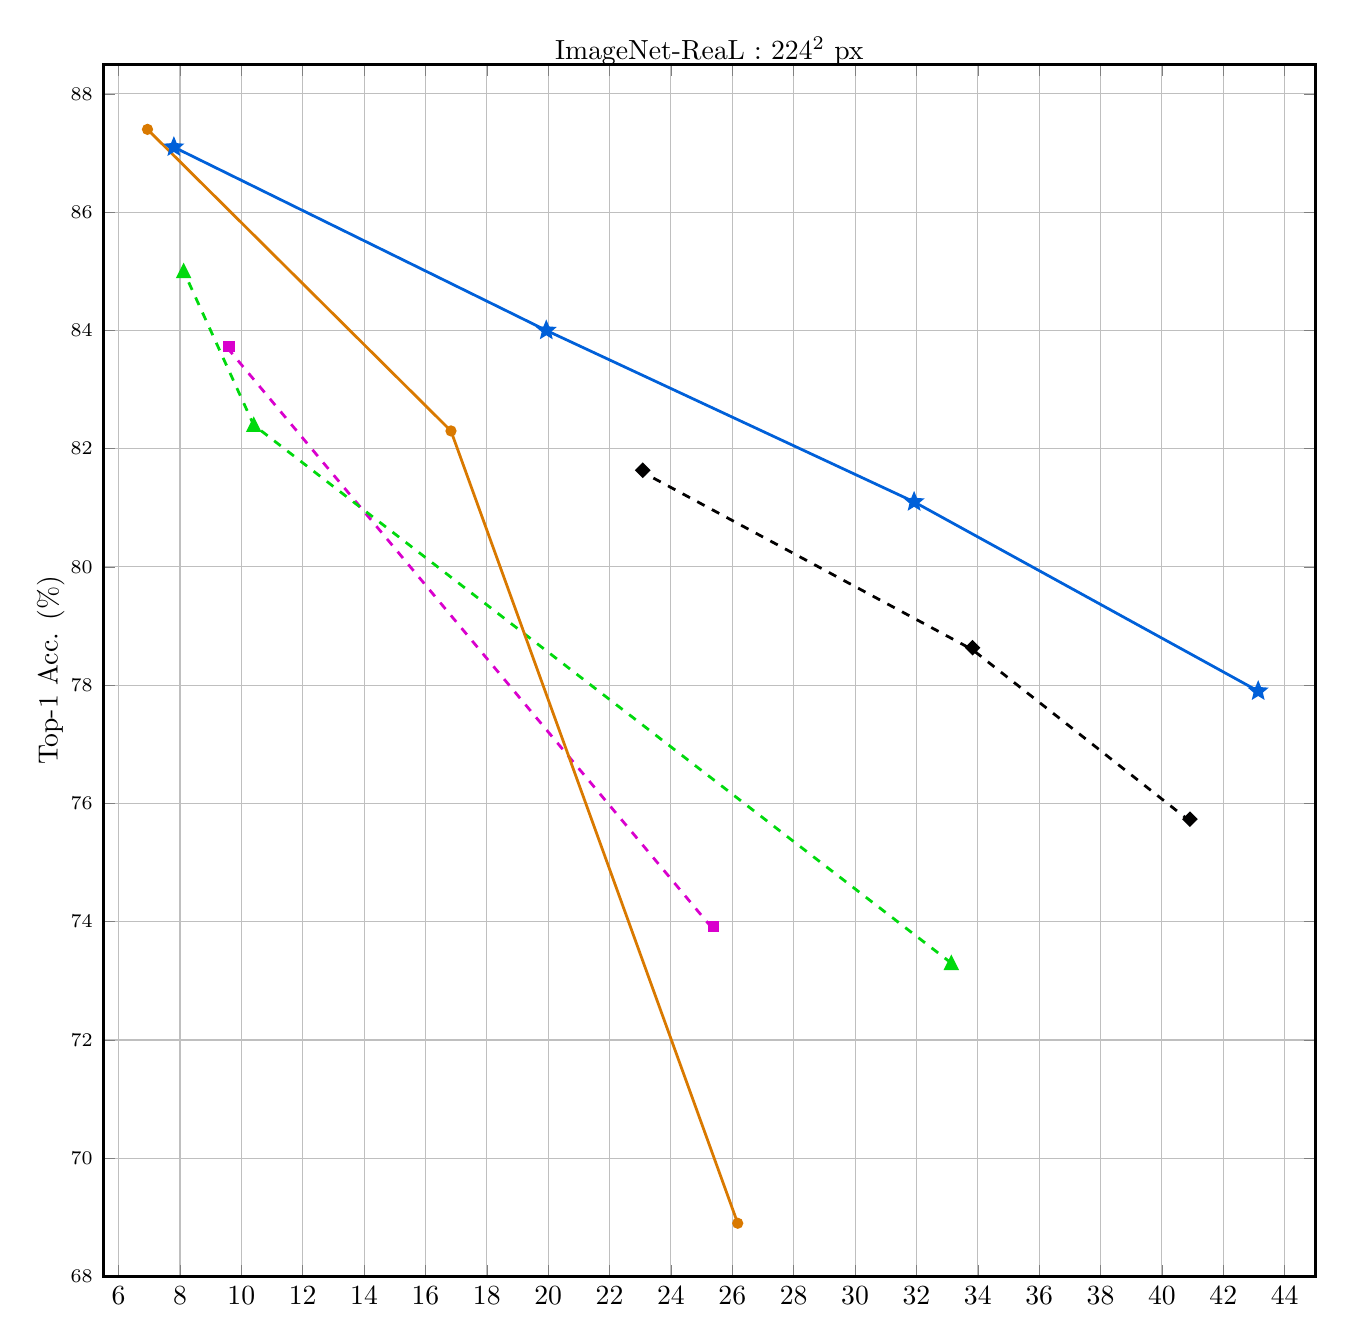
\begin{tikzpicture}
\begin{axis}[
    width=1.4\linewidth,
    height=1.4\linewidth,
    title={ImageNet-ReaL : $224^2$ px},
    title style={yshift=-10pt},
    % xlabel={Throughput (thousand images/s)},
    ylabel={Top-1 Acc. ($\%$)},
    ylabel shift=-5pt,
    xmin=5.5, xmax=45,
    ymin=68, ymax=88.5,
    grid=major,
    line width=1pt,
    yticklabel style={font=\scriptsize},
    xlabel style={font=\footnotesize}
]
% \shade[
%     right color=yellow!60,
%     left color=white,
%     middle color=white,
%     samples=100,
%     opacity=0.2
% ] (rel axis cs:0,1) -- (rel axis cs:1,1) -- (rel axis cs:1,0) -- cycle;

% \shade[
%     top color=yellow!60,
%     bottom color=white,
%     middle color=white,
%     samples=100,
%     opacity=0.2
% ] (rel axis cs:0,1) -- (rel axis cs:1,1) -- (rel axis cs:1,0) -- cycle;

% \node[anchor=south west] at (rel axis cs:0.72,0.87) {\scriptsize optimal};
% ------------------------------------------------------
% 1) EFFICIENTVIT (ICCV 2023)
% ------------------------------------------------------
\draw[\efficientColor, line width=1pt, style=dashed]
  (axis cs:25.328, 73.9) coordinate (B1)
  -- (axis cs:9.553, 83.7) coordinate (B2);

\EfficientMarker[0.5]{(B1)}
\EfficientMarker[0.5]{(B2)}


% ------------------------------------------------------
% 2) SHVIT (CVPR 2024)
% ------------------------------------------------------
\draw[\shvitColor, line width=1pt, style=dashed]
  (axis cs:40.913, 75.7) coordinate (S1)
  -- (axis cs:33.828, 78.6) coordinate (S2)
  -- (axis cs:23.081, 81.6) coordinate (S3);

\ShvitMarker[0.5]{(S1)}
\ShvitMarker[0.5]{(S2)}
\ShvitMarker[0.5]{(S3)}

% ------------------------------------------------------
% 3) MOBILENETV4 (ECCV 2024)
% ------------------------------------------------------
\draw[\mobileColor, line width=1pt, style=dashed]
  (axis cs:33.136, 73.3) coordinate (M1)
  -- (axis cs:10.403, 82.4)  coordinate (M2)
  -- (axis cs:8.121, 85.0)  coordinate (M3);

\MobileMarker[1.0]{(M1)}
\MobileMarker[1.0]{(M2)}
\MobileMarker[1.0]{(M3)}

% ------------------------------------------------------
% 4) VIT+REGISTERS (ICLR 2024)
% ------------------------------------------------------
\draw[\registerColor, line width=1pt]
  (axis cs:26.176, 68.9) coordinate (R1)
  -- (axis cs:16.832, 82.3)  coordinate (R2)
  -- (axis cs:6.942, 87.4)  coordinate (R3);

\RegisterMarker[0.5]{(R1)}
\RegisterMarker[0.5]{(R2)}
\RegisterMarker[0.5]{(R3)}

% ------------------------------------------------------
% 5) VIT+JUMBO (ours)
% ------------------------------------------------------
\draw[\jumboColor, line width=1pt]
  (axis cs:43.137,77.9) coordinate (J0)
  -- (axis cs:31.924,81.1) coordinate (J1)
  -- (axis cs:19.938,84.0) coordinate (J2)
  -- (axis cs:7.802,87.1) coordinate (J3);

\JumboMarker[0.25]{(J0)}
\JumboMarker[0.25]{(J1)}
\JumboMarker[0.25]{(J2)}
\JumboMarker[0.25]{(J3)}

\end{axis}
\end{tikzpicture}

        \phantomcaption
        \label{fig:sub:plot5}
    \end{subfigure}
    \hspace{0.7cm}
    \begin{subfigure}[b]{0.22\textwidth}
        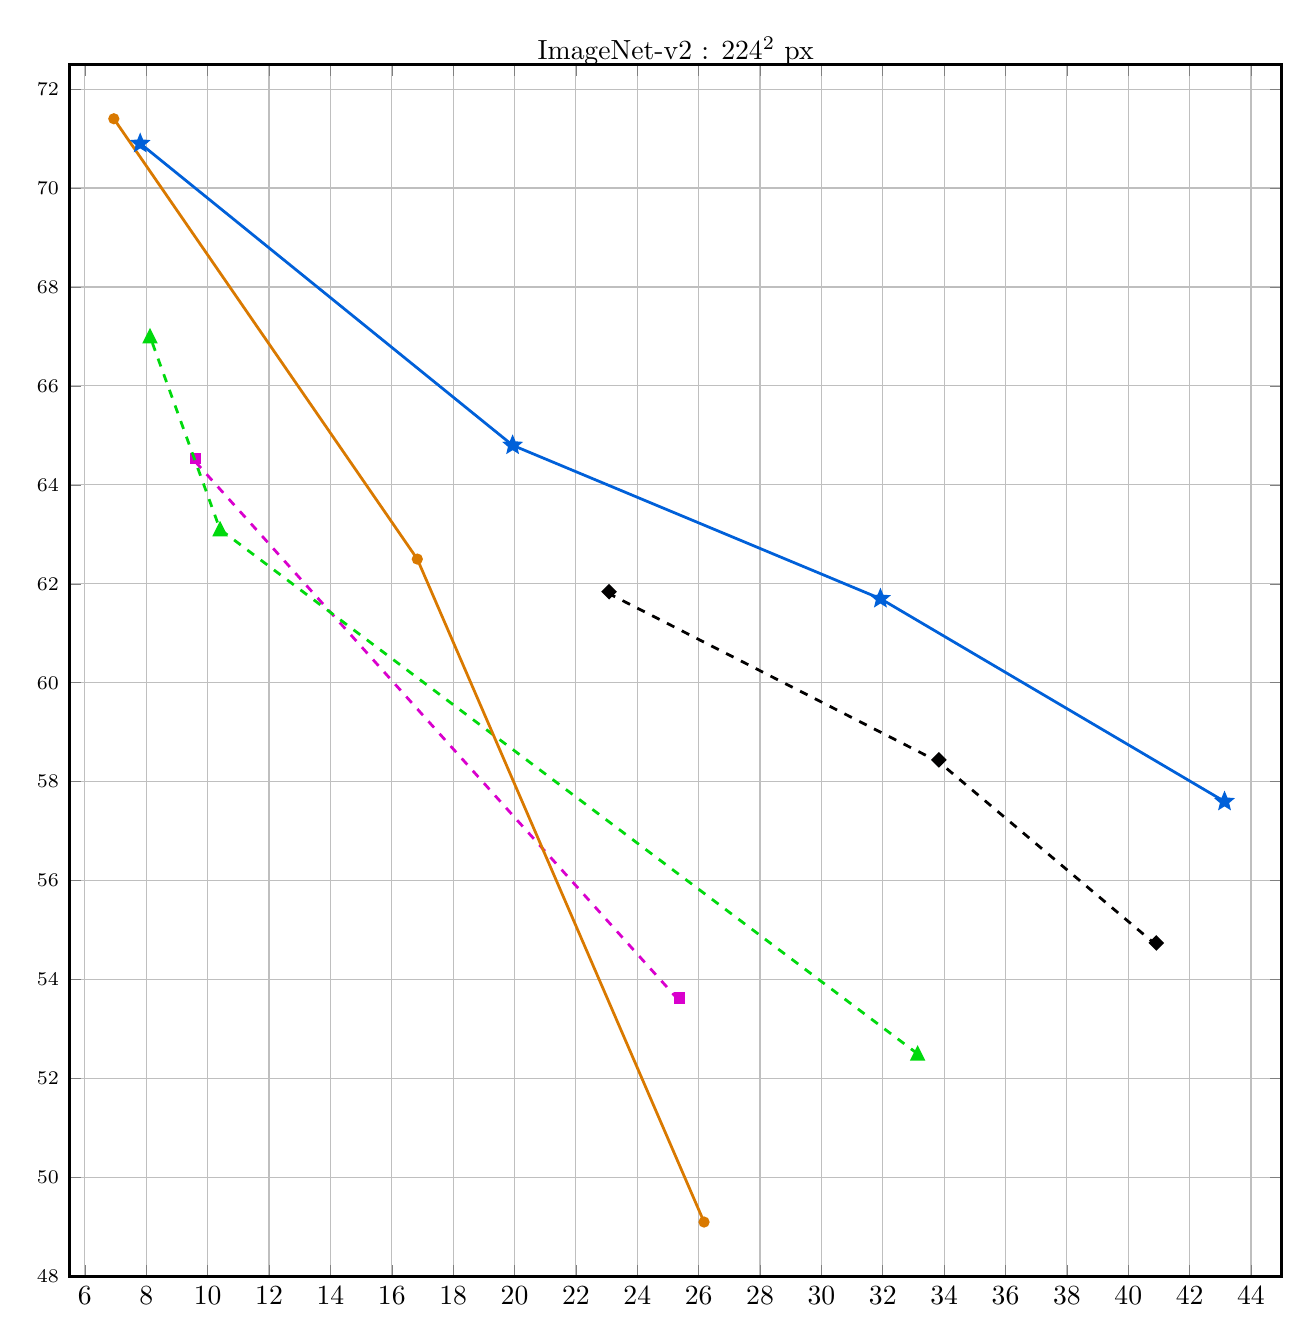
\begin{tikzpicture}
\begin{axis}[
    width=1.4\linewidth,
    height=1.4\linewidth,
    title={ImageNet-v2 : $224^2$ px},
    title style={yshift=-10pt},
    % xlabel={Throughput (thousand images/s)},
    ylabel shift=-5pt,
    xmin=5.5, xmax=45,
    ymin=48, ymax=72.5,
    grid=major,
    line width=1pt,
    yticklabel style={font=\scriptsize},
    xlabel style={font=\footnotesize}
]
% \shade[
%     right color=yellow!60,
%     left color=white,
%     middle color=white,
%     samples=100,
%     opacity=0.2
% ] (rel axis cs:0,1) -- (rel axis cs:1,1) -- (rel axis cs:1,0) -- cycle;

% \shade[
%     top color=yellow!60,
%     bottom color=white,
%     middle color=white,
%     samples=100,
%     opacity=0.2
% ] (rel axis cs:0,1) -- (rel axis cs:1,1) -- (rel axis cs:1,0) -- cycle;

% \node[anchor=south west] at (rel axis cs:0.72,0.87) {\scriptsize optimal};
% ------------------------------------------------------
% 1) EFFICIENTVIT (ICCV 2023)
% ------------------------------------------------------
\draw[\efficientColor, line width=1pt, style=dashed]
  (axis cs:25.328, 53.6) coordinate (B1)
  -- (axis cs:9.553, 64.5) coordinate (B2);

\EfficientMarker[0.5]{(B1)}
\EfficientMarker[0.5]{(B2)}
% ------------------------------------------------------
% 2) SHVIT (CVPR 2024)
% ------------------------------------------------------
\draw[\shvitColor, line width=1pt, style=dashed]
  (axis cs:40.913, 54.7) coordinate (S1)
  -- (axis cs:33.828, 58.4) coordinate (S2)
  -- (axis cs:23.081, 61.8) coordinate (S3);

\ShvitMarker[0.5]{(S1)}
\ShvitMarker[0.5]{(S2)}
\ShvitMarker[0.5]{(S3)}

% ------------------------------------------------------
% 3) MOBILENETV4 (ECCV 2024)
% ------------------------------------------------------
\draw[\mobileColor, line width=1pt, style=dashed]
  (axis cs:33.136, 52.5) coordinate (M1)
  -- (axis cs:10.403, 63.1)  coordinate (M2)
  -- (axis cs:8.121, 67.0)  coordinate (M3);

\MobileMarker[1.0]{(M1)}
\MobileMarker[1.0]{(M2)}
\MobileMarker[1.0]{(M3)}

% ------------------------------------------------------
% 4) VIT+REGISTERS (ICLR 2024)
% ------------------------------------------------------
\draw[\registerColor, line width=1pt]
  (axis cs:26.176, 49.1) coordinate (R1)
  -- (axis cs:16.832, 62.5)  coordinate (R2)
  -- (axis cs:6.942, 71.4)  coordinate (R3);

\RegisterMarker[0.5]{(R1)}
\RegisterMarker[0.5]{(R2)}
\RegisterMarker[0.5]{(R3)}

% ------------------------------------------------------
% 5) VIT+JUMBO (ours)
% ------------------------------------------------------
\draw[\jumboColor, line width=1pt]
  (axis cs:43.137,57.6) coordinate (J0)
  -- (axis cs:31.924,61.7) coordinate (J1)
  -- (axis cs:19.938,64.8) coordinate (J2)
  -- (axis cs:7.802,70.9) coordinate (J3);

\JumboMarker[0.25]{(J0)}
\JumboMarker[0.25]{(J1)}
\JumboMarker[0.25]{(J2)}
\JumboMarker[0.25]{(J3)}

\end{axis}
\end{tikzpicture}

        \phantomcaption
        \label{fig:sub:plot6}
    \end{subfigure}
    \hspace{0.3cm}
    \begin{subfigure}[b]{0.22\textwidth}
        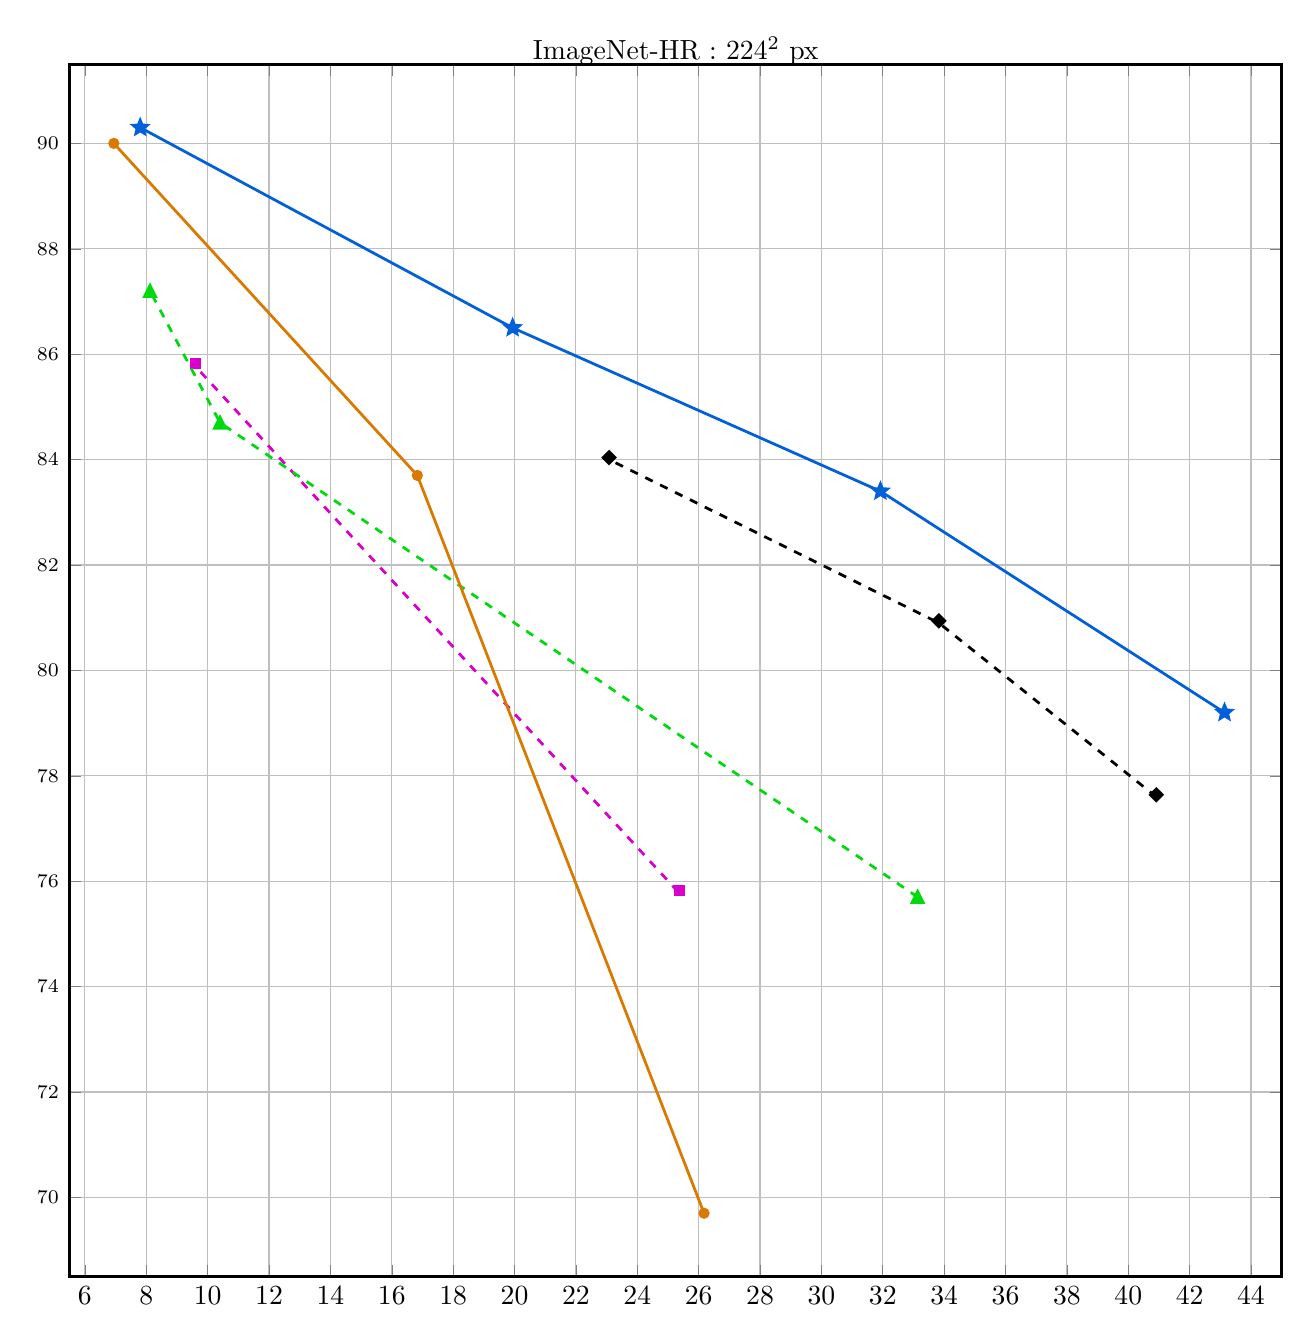
\begin{tikzpicture}
\begin{axis}[
    width=1.4\linewidth,
    height=1.4\linewidth,
    title={ImageNet-HR : $224^2$ px},
    title style={yshift=-10pt},
    % xlabel={Throughput (thousand images/s)},
    ylabel shift=-5pt,
    xmin=5.5, xmax=45,
    ymin=68.5, ymax=91.5,
    grid=major,
    line width=1pt,
    yticklabel style={font=\scriptsize},
    xlabel style={font=\footnotesize}
]
% \shade[
%     right color=yellow!60,
%     left color=white,
%     middle color=white,
%     samples=100,
%     opacity=0.2
% ] (rel axis cs:0,1) -- (rel axis cs:1,1) -- (rel axis cs:1,0) -- cycle;

% \shade[
%     top color=yellow!60,
%     bottom color=white,
%     middle color=white,
%     samples=100,
%     opacity=0.2
% ] (rel axis cs:0,1) -- (rel axis cs:1,1) -- (rel axis cs:1,0) -- cycle;

% \node[anchor=south west] at (rel axis cs:0.72,0.87) {\scriptsize optimal};
% ------------------------------------------------------
% 1) EFFICIENTVIT (ICCV 2023)
% ------------------------------------------------------
\draw[\efficientColor, line width=1pt, style=dashed]
  (axis cs:25.328, 75.8) coordinate (B1)
  -- (axis cs:9.553, 85.8) coordinate (B2);

\EfficientMarker[0.5]{(B1)}
\EfficientMarker[0.5]{(B2)}

% ------------------------------------------------------
% 2) SHVIT (CVPR 2024)
% ------------------------------------------------------
\draw[\shvitColor, line width=1pt, style=dashed]
  (axis cs:40.913, 77.6) coordinate (S1)
  -- (axis cs:33.828, 80.9) coordinate (S2)
  -- (axis cs:23.081, 84.0) coordinate (S3);

\ShvitMarker[0.5]{(S1)}
\ShvitMarker[0.5]{(S2)}
\ShvitMarker[0.5]{(S3)}

% ------------------------------------------------------
% 3) MOBILENETV4 (ECCV 2024)
% ------------------------------------------------------
\draw[\mobileColor, line width=1pt, style=dashed]
  (axis cs:33.136, 75.7) coordinate (M1)
  -- (axis cs:10.403, 84.7)  coordinate (M2)
  -- (axis cs:8.121, 87.2)  coordinate (M3);

\MobileMarker[1.0]{(M1)}
\MobileMarker[1.0]{(M2)}
\MobileMarker[1.0]{(M3)}

% ------------------------------------------------------
% 4) VIT+REGISTERS (ICLR 2024)
% ------------------------------------------------------
\draw[\registerColor, line width=1pt]
  (axis cs:26.176, 69.7) coordinate (R1)
  -- (axis cs:16.832, 83.7)  coordinate (R2)
  -- (axis cs:6.942, 90.0)  coordinate (R3);

\RegisterMarker[0.5]{(R1)}
\RegisterMarker[0.5]{(R2)}
\RegisterMarker[0.5]{(R3)}

% ------------------------------------------------------
% 5) VIT+JUMBO (ours)
% ------------------------------------------------------
\draw[\jumboColor, line width=1pt]
  (axis cs:43.137,79.2) coordinate (J0)
  -- (axis cs:31.924,83.4) coordinate (J1)
  -- (axis cs:19.938,86.5) coordinate (J2)
  -- (axis cs:7.802,90.3) coordinate (J3);

\JumboMarker[0.25]{(J0)}
\JumboMarker[0.25]{(J1)}
\JumboMarker[0.25]{(J2)}
\JumboMarker[0.25]{(J3)}

\end{axis}
\end{tikzpicture}

        \phantomcaption
        \label{fig:sub:plot7}
    \end{subfigure}
    \hspace{0.3cm}
    \begin{subfigure}[b]{0.22\textwidth}
        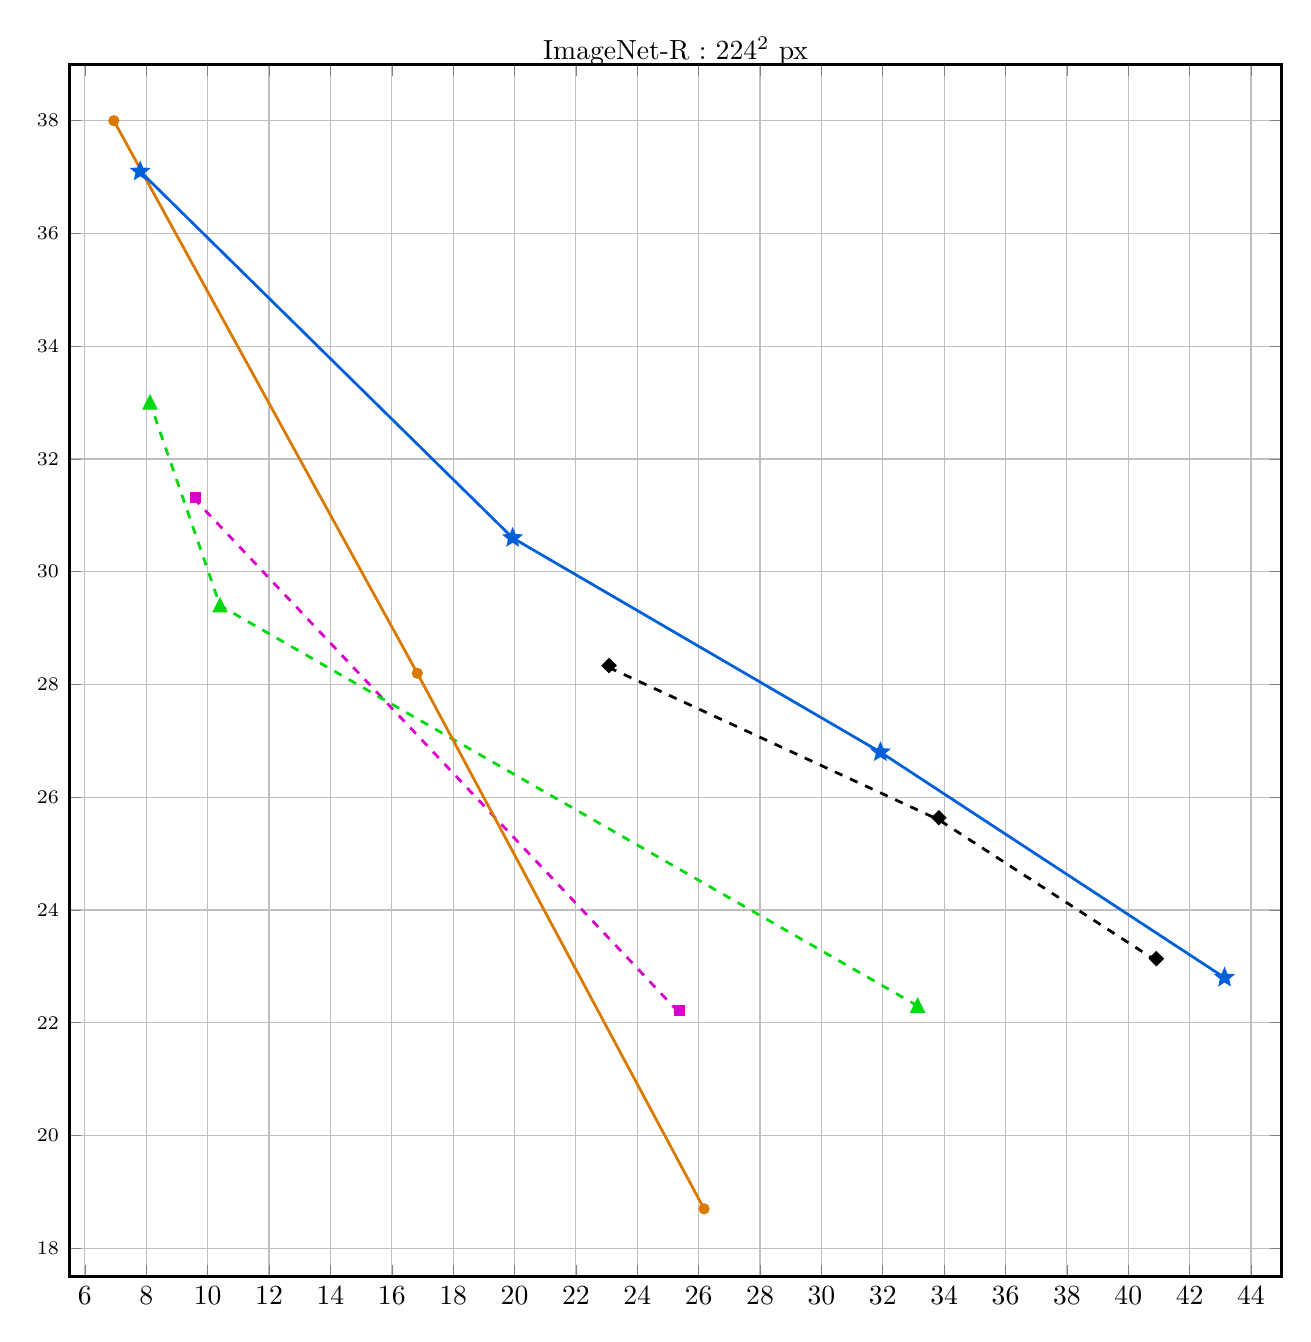
\begin{tikzpicture}
\begin{axis}[
    width=1.4\linewidth,
    height=1.4\linewidth,
    title={ImageNet-R : $224^2$ px},
    title style={yshift=-10pt},
    % xlabel={Throughput (thousand images/s)},
    ylabel shift=-5pt,
    xmin=5.5, xmax=45,
    ymin=17.5, ymax=39,
    grid=major,
    line width=1pt,
    yticklabel style={font=\scriptsize},
    xlabel style={font=\footnotesize}
]
% \shade[
%     right color=yellow!60,
%     left color=white,
%     middle color=white,
%     samples=100,
%     opacity=0.2
% ] (rel axis cs:0,1) -- (rel axis cs:1,1) -- (rel axis cs:1,0) -- cycle;

% \shade[
%     top color=yellow!60,
%     bottom color=white,
%     middle color=white,
%     samples=100,
%     opacity=0.2
% ] (rel axis cs:0,1) -- (rel axis cs:1,1) -- (rel axis cs:1,0) -- cycle;

% \node[anchor=south west] at (rel axis cs:0.72,0.87) {\scriptsize optimal};
% ------------------------------------------------------
% 1) EFFICIENTVIT (ICCV 2023)
% ------------------------------------------------------
\draw[\efficientColor, line width=1pt, style=dashed]
  (axis cs:25.328, 22.2) coordinate (B1)
  -- (axis cs:9.553, 31.3) coordinate (B2);

\EfficientMarker[0.5]{(B1)}
\EfficientMarker[0.5]{(B2)}


% ------------------------------------------------------
% 2) SHVIT (CVPR 2024)
% ------------------------------------------------------
\draw[\shvitColor, line width=1pt, style=dashed]
  (axis cs:40.913, 23.1) coordinate (S1)
  -- (axis cs:33.828, 25.6) coordinate (S2)
  -- (axis cs:23.081, 28.3) coordinate (S3);

\ShvitMarker[0.5]{(S1)}
\ShvitMarker[0.5]{(S2)}
\ShvitMarker[0.5]{(S3)}

% ------------------------------------------------------
% 3) MOBILENETV4 (ECCV 2024)
% ------------------------------------------------------
\draw[\mobileColor, line width=1pt, style=dashed]
  (axis cs:33.136, 22.3) coordinate (M1)
  -- (axis cs:10.403, 29.4)  coordinate (M2)
  -- (axis cs:8.121, 33.0)  coordinate (M3);

\MobileMarker[1.0]{(M1)}
\MobileMarker[1.0]{(M2)}
\MobileMarker[1.0]{(M3)}

% ------------------------------------------------------
% 4) VIT+REGISTERS (ICLR 2024)
% ------------------------------------------------------
\draw[\registerColor, line width=1pt]
  (axis cs:26.176, 18.7) coordinate (R1)
  -- (axis cs:16.832, 28.2)  coordinate (R2)
  -- (axis cs:6.942, 38.0)  coordinate (R3);

\RegisterMarker[0.5]{(R1)}
\RegisterMarker[0.5]{(R2)}
\RegisterMarker[0.5]{(R3)}

% ------------------------------------------------------
% 5) VIT+JUMBO (ours)
% ------------------------------------------------------
\draw[\jumboColor, line width=1pt]
  (axis cs:43.137,22.8) coordinate (J0)
  -- (axis cs:31.924,26.8) coordinate (J1)
  -- (axis cs:19.938,30.6) coordinate (J2)
  -- (axis cs:7.802,37.1) coordinate (J3);

\JumboMarker[0.25]{(J0)}
\JumboMarker[0.25]{(J1)}
\JumboMarker[0.25]{(J2)}
\JumboMarker[0.25]{(J3)}

\end{axis}
\end{tikzpicture}

        \phantomcaption
        \label{fig:sub:plot8}
    \end{subfigure}
    
    \vspace{-0.5cm}
    
    %-------------------------------------------------
    % Second row of plots
    %-------------------------------------------------
    \hspace{-0.6cm}
    \begin{subfigure}[b]{0.22\textwidth}
        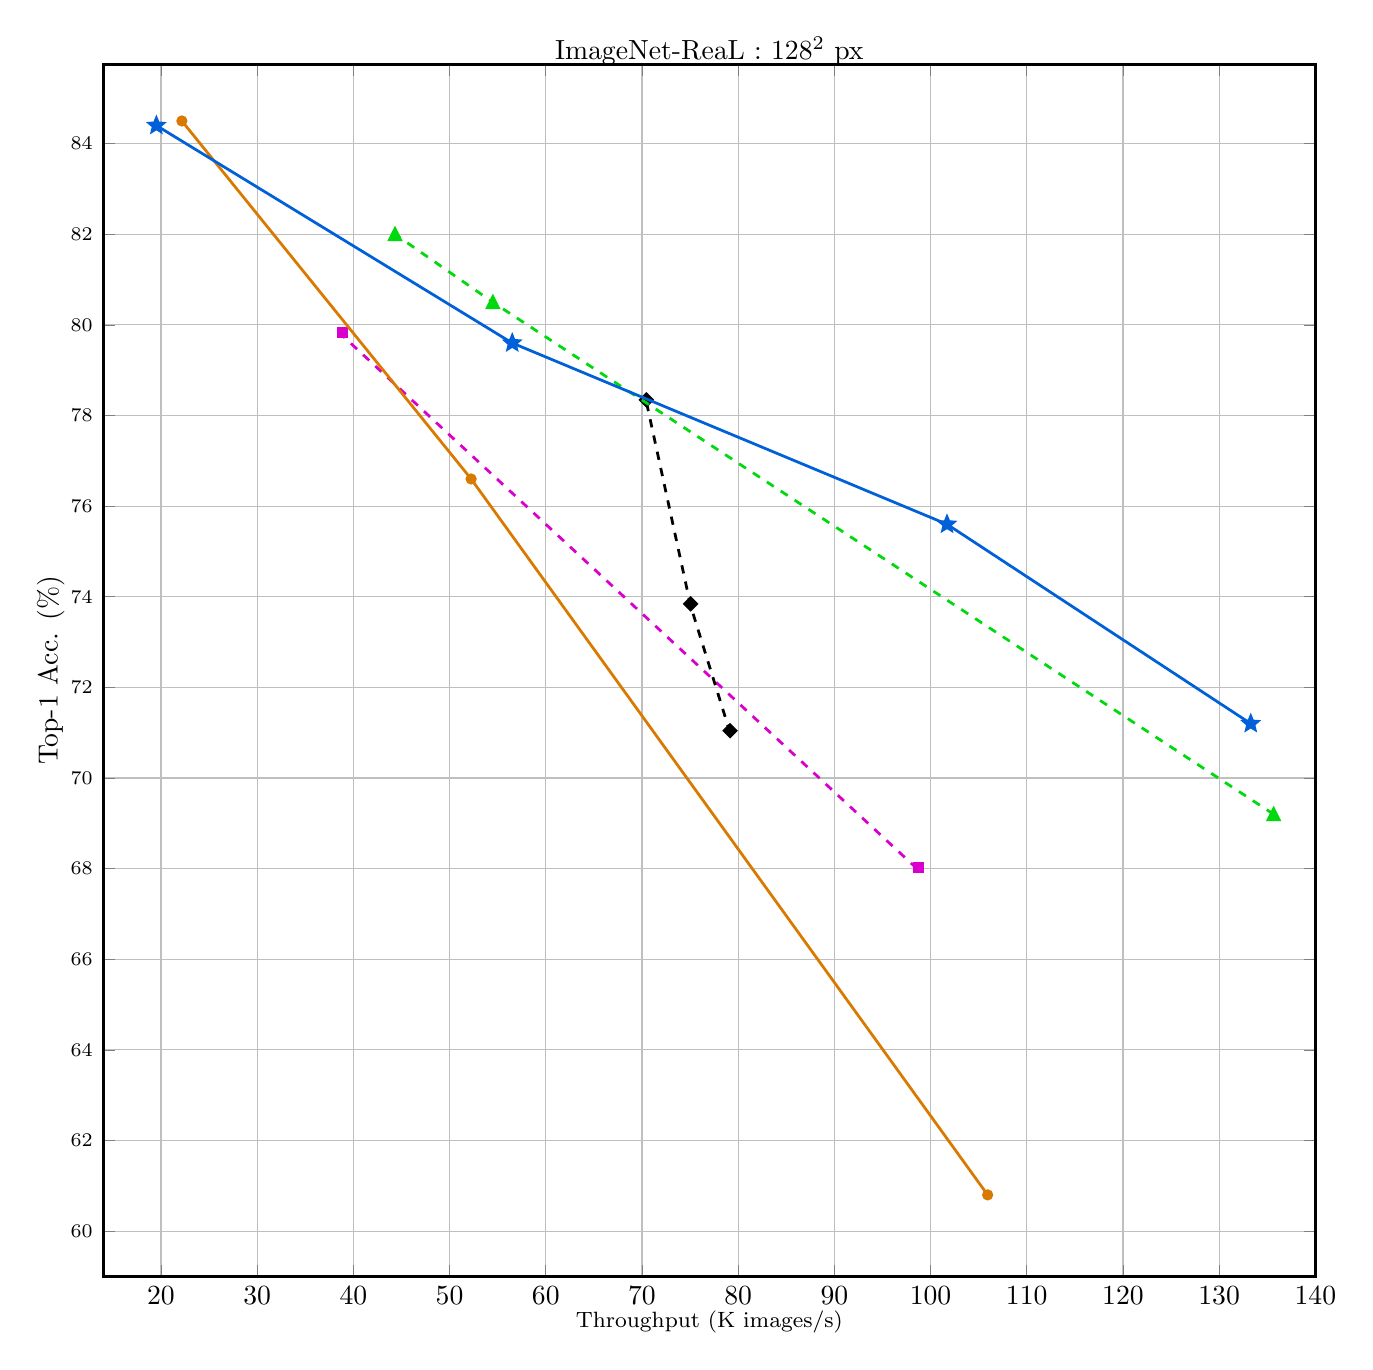
\begin{tikzpicture}
\begin{axis}[
    width=1.4\linewidth,
    height=1.4\linewidth,
    title={ImageNet-ReaL : $128^2$ px},
    title style={yshift=-10pt},
    xlabel={Throughput (K images/s)},
    ylabel={Top-1 Acc. ($\%$)},
    ylabel shift=-5pt,
    xlabel shift=-5pt,
    xmin=14, xmax=140,
    ymin=59, ymax=85.75,
    grid=major,
    line width=1pt,
    yticklabel style={font=\scriptsize},
    xlabel style={font=\footnotesize}
]
% \shade[
%     right color=yellow!60,
%     left color=white,
%     middle color=white,
%     samples=100,
%     opacity=0.2
% ] (rel axis cs:0,1) -- (rel axis cs:1,1) -- (rel axis cs:1,0) -- cycle;

% \shade[
%     top color=yellow!60,
%     bottom color=white,
%     middle color=white,
%     samples=100,
%     opacity=0.2
% ] (rel axis cs:0,1) -- (rel axis cs:1,1) -- (rel axis cs:1,0) -- cycle;

% \node[anchor=south west] at (rel axis cs:0.72,0.87) {\scriptsize optimal};
% ------------------------------------------------------
% 1) EFFICIENTVIT (ICCV 2023)
% ------------------------------------------------------
\draw[\efficientColor, line width=1pt, style=dashed]
  (axis cs:98.585, 68.0) coordinate (B1)
  -- (axis cs:38.683, 79.8) coordinate (B2);
  % node[midway, above, sloped] {\small ViT+Registers};

\EfficientMarker[0.5]{(B1)}
% \node[below, \efficientColor] at (B1) {\small small};

\EfficientMarker[0.5]{(B2)}
% \node[above, \efficientColor] at (B2) {\small base};


% ------------------------------------------------------
% 2) SHVIT (CVPR 2024)
% ------------------------------------------------------
\draw[\shvitColor, line width=1pt, style=dashed]
  (axis cs:79.163, 71.0) coordinate (S1)
  -- (axis cs:75.060, 73.8) coordinate (S2)
  -- (axis cs:70.458, 78.3) coordinate (S3);

\ShvitMarker[0.5]{(S1)}
\ShvitMarker[0.5]{(S2)}
\ShvitMarker[0.5]{(S3)}

% ------------------------------------------------------
% 3) MOBILENETV4 (ECCV 2024)
% ------------------------------------------------------
\draw[\mobileColor, line width=1pt, style=dashed]
  (axis cs:135.663, 69.2) coordinate (M1)
  -- (axis cs:54.500, 80.5)  coordinate (M2)
  -- (axis cs:44.325, 82.0)  coordinate (M3);

\MobileMarker[1.0]{(M1)}
\MobileMarker[1.0]{(M2)}
\MobileMarker[1.0]{(M3)}

% ------------------------------------------------------
% 4) VIT+REGISTERS (ICLR 2024)
% ------------------------------------------------------
\draw[\registerColor, line width=1pt]
  (axis cs:105.933, 60.8) coordinate (R1)
  -- (axis cs:52.241, 76.6)  coordinate (R2)
  -- (axis cs:22.176, 84.5)  coordinate (R3);

\RegisterMarker[0.5]{(R1)}
\RegisterMarker[0.5]{(R2)}
\RegisterMarker[0.5]{(R3)}

% ------------------------------------------------------
% 5) VIT+JUMBO (ours)
% ------------------------------------------------------
\draw[\jumboColor, line width=1pt]
  (axis cs:133.285,71.2) coordinate (J0)
  -- (axis cs:101.711,75.6) coordinate (J1)
  -- (axis cs:56.516,79.6) coordinate (J2)
  -- (axis cs:19.524,84.4) coordinate (J3);

\JumboMarker[0.25]{(J0)}
\JumboMarker[0.25]{(J1)}
\JumboMarker[0.25]{(J2)}
\JumboMarker[0.25]{(J3)}

\end{axis}
\end{tikzpicture}

        \phantomcaption
        \label{fig:sub:plot1}
    \end{subfigure}
    \hspace{0.7cm}
    \begin{subfigure}[b]{0.22\textwidth}
        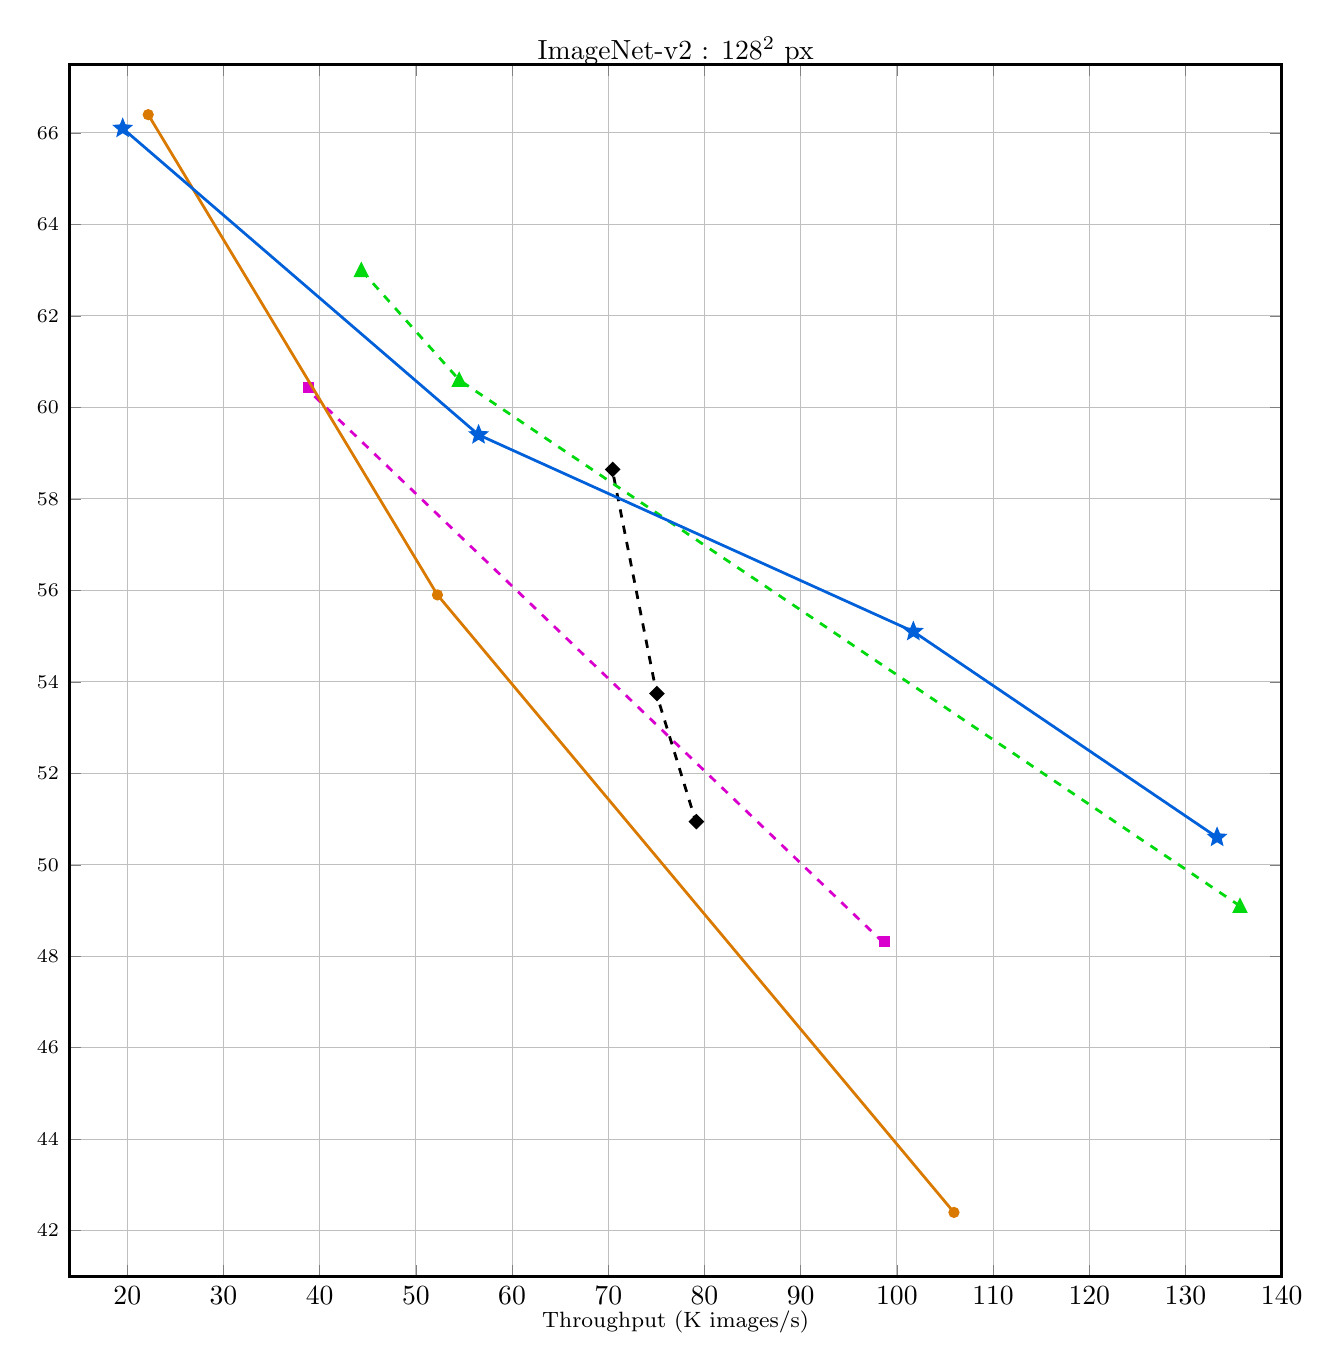
\begin{tikzpicture}
\begin{axis}[
    width=1.4\linewidth,
    height=1.4\linewidth,
    title={ImageNet-v2 : $128^2$ px},
    title style={yshift=-10pt},
    xlabel={Throughput (K images/s)},
    ylabel shift=-5pt,
    xlabel shift=-5pt,
    xmin=14, xmax=140,
    ymin=41, ymax=67.5,
    grid=major,
    line width=1pt,
    yticklabel style={font=\scriptsize},
    xlabel style={font=\footnotesize}
]
% \shade[
%     right color=yellow!60,
%     left color=white,
%     middle color=white,
%     samples=100,
%     opacity=0.2
% ] (rel axis cs:0,1) -- (rel axis cs:1,1) -- (rel axis cs:1,0) -- cycle;

% \shade[
%     top color=yellow!60,
%     bottom color=white,
%     middle color=white,
%     samples=100,
%     opacity=0.2
% ] (rel axis cs:0,1) -- (rel axis cs:1,1) -- (rel axis cs:1,0) -- cycle;

% \node[anchor=south west] at (rel axis cs:0.72,0.87) {\scriptsize optimal};
% ------------------------------------------------------
% 1) EFFICIENTVIT (ICCV 2023)
% ------------------------------------------------------
\draw[\efficientColor, line width=1pt, style=dashed]
  (axis cs:98.585, 48.3) coordinate (B1)
  -- (axis cs:38.683, 60.4) coordinate (B2);

\EfficientMarker[0.5]{(B1)}
\EfficientMarker[0.5]{(B2)}

% ------------------------------------------------------
% 2) SHVIT (CVPR 2024)
% ------------------------------------------------------
\draw[\shvitColor, line width=1pt, style=dashed]
  (axis cs:79.163, 50.9) coordinate (S1)
  -- (axis cs:75.060, 53.7) coordinate (S2)
  -- (axis cs:70.458, 58.6) coordinate (S3);

\ShvitMarker[0.5]{(S1)}
\ShvitMarker[0.5]{(S2)}
\ShvitMarker[0.5]{(S3)}

% ------------------------------------------------------
% 3) MOBILENETV4 (ECCV 2024)
% ------------------------------------------------------
\draw[\mobileColor, line width=1pt, style=dashed]
  (axis cs:135.663, 49.1) coordinate (M1)
  -- (axis cs:54.500, 60.6)  coordinate (M2)
  -- (axis cs:44.325, 63.0)  coordinate (M3);

\MobileMarker[1.0]{(M1)}
\MobileMarker[1.0]{(M2)}
\MobileMarker[1.0]{(M3)}

% ------------------------------------------------------
% 4) VIT+REGISTERS (ICLR 2024)
% ------------------------------------------------------
\draw[\registerColor, line width=1pt]
  (axis cs:105.933, 42.4) coordinate (R1)
  -- (axis cs:52.241, 55.9)  coordinate (R2)
  -- (axis cs:22.176, 66.4)  coordinate (R3);

\RegisterMarker[0.5]{(R1)}
\RegisterMarker[0.5]{(R2)}
\RegisterMarker[0.5]{(R3)}

% ------------------------------------------------------
% 5) VIT+JUMBO (ours)
% ------------------------------------------------------
\draw[\jumboColor, line width=1pt]
  (axis cs:133.285,50.6) coordinate (J0)
  -- (axis cs:101.711, 55.1) coordinate (J1)
  -- (axis cs:56.516, 59.4) coordinate (J2)
  -- (axis cs:19.524, 66.1) coordinate (J3);

\JumboMarker[0.25]{(J0)}
\JumboMarker[0.25]{(J1)}
\JumboMarker[0.25]{(J2)}
\JumboMarker[0.25]{(J3)}

\end{axis}
\end{tikzpicture}

        \phantomcaption
        \label{fig:sub:plot2}
    \end{subfigure}
    \hspace{0.3cm}
    \begin{subfigure}[b]{0.22\textwidth}
        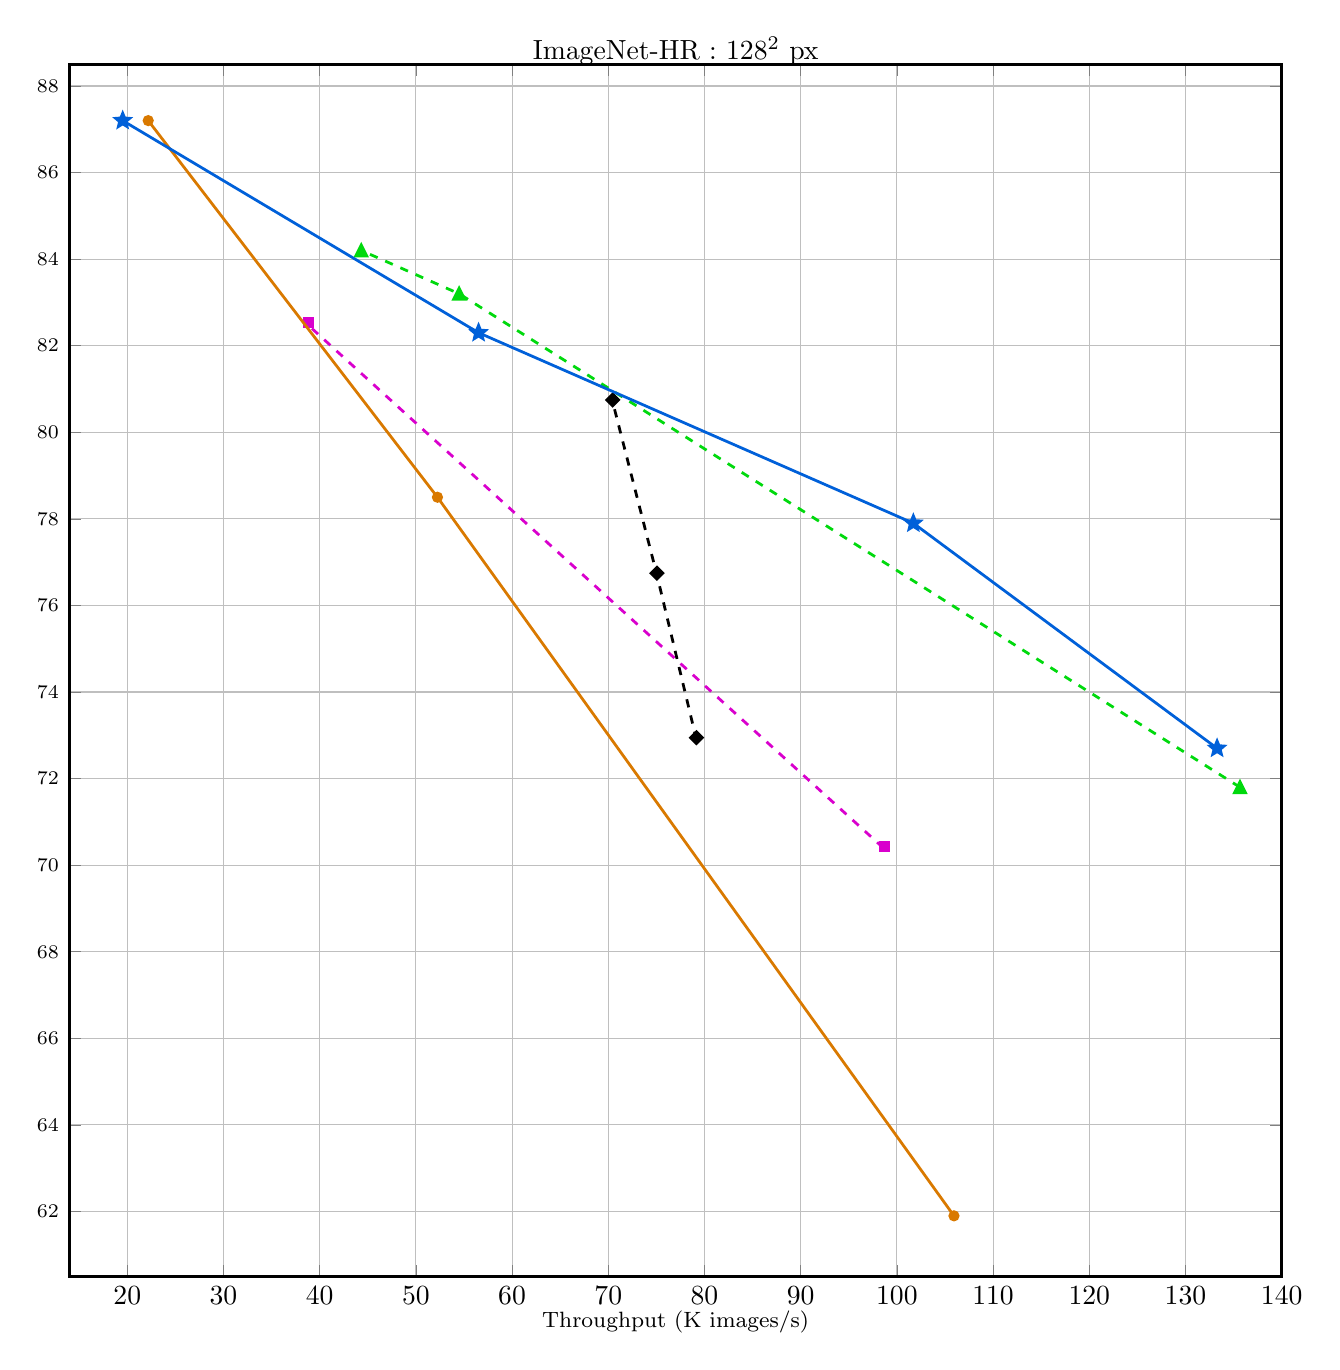
\begin{tikzpicture}
\begin{axis}[
    width=1.4\linewidth,
    height=1.4\linewidth,
    title={ImageNet-HR : $128^2$ px},
    title style={yshift=-10pt},
    xlabel={Throughput (K images/s)},
    ylabel shift=-5pt,
    xlabel shift=-5pt,
    xmin=14, xmax=140,
    ymin=60.5, ymax=88.5,
    grid=major,
    line width=1pt,
    yticklabel style={font=\scriptsize},
    xlabel style={font=\footnotesize}
]
% \shade[
%     right color=yellow!60,
%     left color=white,
%     middle color=white,
%     samples=100,
%     opacity=0.2
% ] (rel axis cs:0,1) -- (rel axis cs:1,1) -- (rel axis cs:1,0) -- cycle;

% \shade[
%     top color=yellow!60,
%     bottom color=white,
%     middle color=white,
%     samples=100,
%     opacity=0.2
% ] (rel axis cs:0,1) -- (rel axis cs:1,1) -- (rel axis cs:1,0) -- cycle;

% \node[anchor=south west] at (rel axis cs:0.72,0.87) {\scriptsize optimal};
% ------------------------------------------------------
% 1) EFFICIENTVIT (ICCV 2023)
% ------------------------------------------------------
\draw[\efficientColor, line width=1pt, style=dashed]
  (axis cs:98.585, 70.4) coordinate (B1)
  -- (axis cs:38.683, 82.5) coordinate (B2);


\EfficientMarker[0.5]{(B1)}
\EfficientMarker[0.5]{(B2)}

% ------------------------------------------------------
% 2) SHVIT (CVPR 2024)
% ------------------------------------------------------
\draw[\shvitColor, line width=1pt, style=dashed]
  (axis cs:79.163, 72.9) coordinate (S1)
  -- (axis cs:75.060, 76.7) coordinate (S2)
  -- (axis cs:70.458, 80.7) coordinate (S3);

\ShvitMarker[0.5]{(S1)}
\ShvitMarker[0.5]{(S2)}
\ShvitMarker[0.5]{(S3)}

% ------------------------------------------------------
% 3) MOBILENETV4 (ECCV 2024)
% ------------------------------------------------------
\draw[\mobileColor, line width=1pt, style=dashed]
  (axis cs:135.663, 71.8) coordinate (M1)
  -- (axis cs:54.500, 83.2)  coordinate (M2)
  -- (axis cs:44.325, 84.2)  coordinate (M3);

\MobileMarker[1.0]{(M1)}
\MobileMarker[1.0]{(M2)}
\MobileMarker[1.0]{(M3)}

% ------------------------------------------------------
% 4) VIT+REGISTERS (ICLR 2024)
% ------------------------------------------------------
\draw[\registerColor, line width=1pt]
  (axis cs:105.933, 61.9) coordinate (R1)
  -- (axis cs:52.241, 78.5)  coordinate (R2)
  -- (axis cs:22.176, 87.2)  coordinate (R3);

\RegisterMarker[0.5]{(R1)}
\RegisterMarker[0.5]{(R2)}
\RegisterMarker[0.5]{(R3)}

% ------------------------------------------------------
% 5) VIT+JUMBO (ours)
% ------------------------------------------------------
\draw[\jumboColor, line width=1pt]
  (axis cs:133.285,72.7) coordinate (J0)
  -- (axis cs:101.711, 77.9) coordinate (J1)
  -- (axis cs:56.516, 82.3) coordinate (J2)
  -- (axis cs:19.524, 87.2) coordinate (J3);

\JumboMarker[0.25]{(J0)}
\JumboMarker[0.25]{(J1)}
\JumboMarker[0.25]{(J2)}
\JumboMarker[0.25]{(J3)}

\end{axis}
\end{tikzpicture}

        \phantomcaption
        \label{fig:sub:plot3}
    \end{subfigure}
    \hspace{0.3cm}
    \begin{subfigure}[b]{0.22\textwidth}
        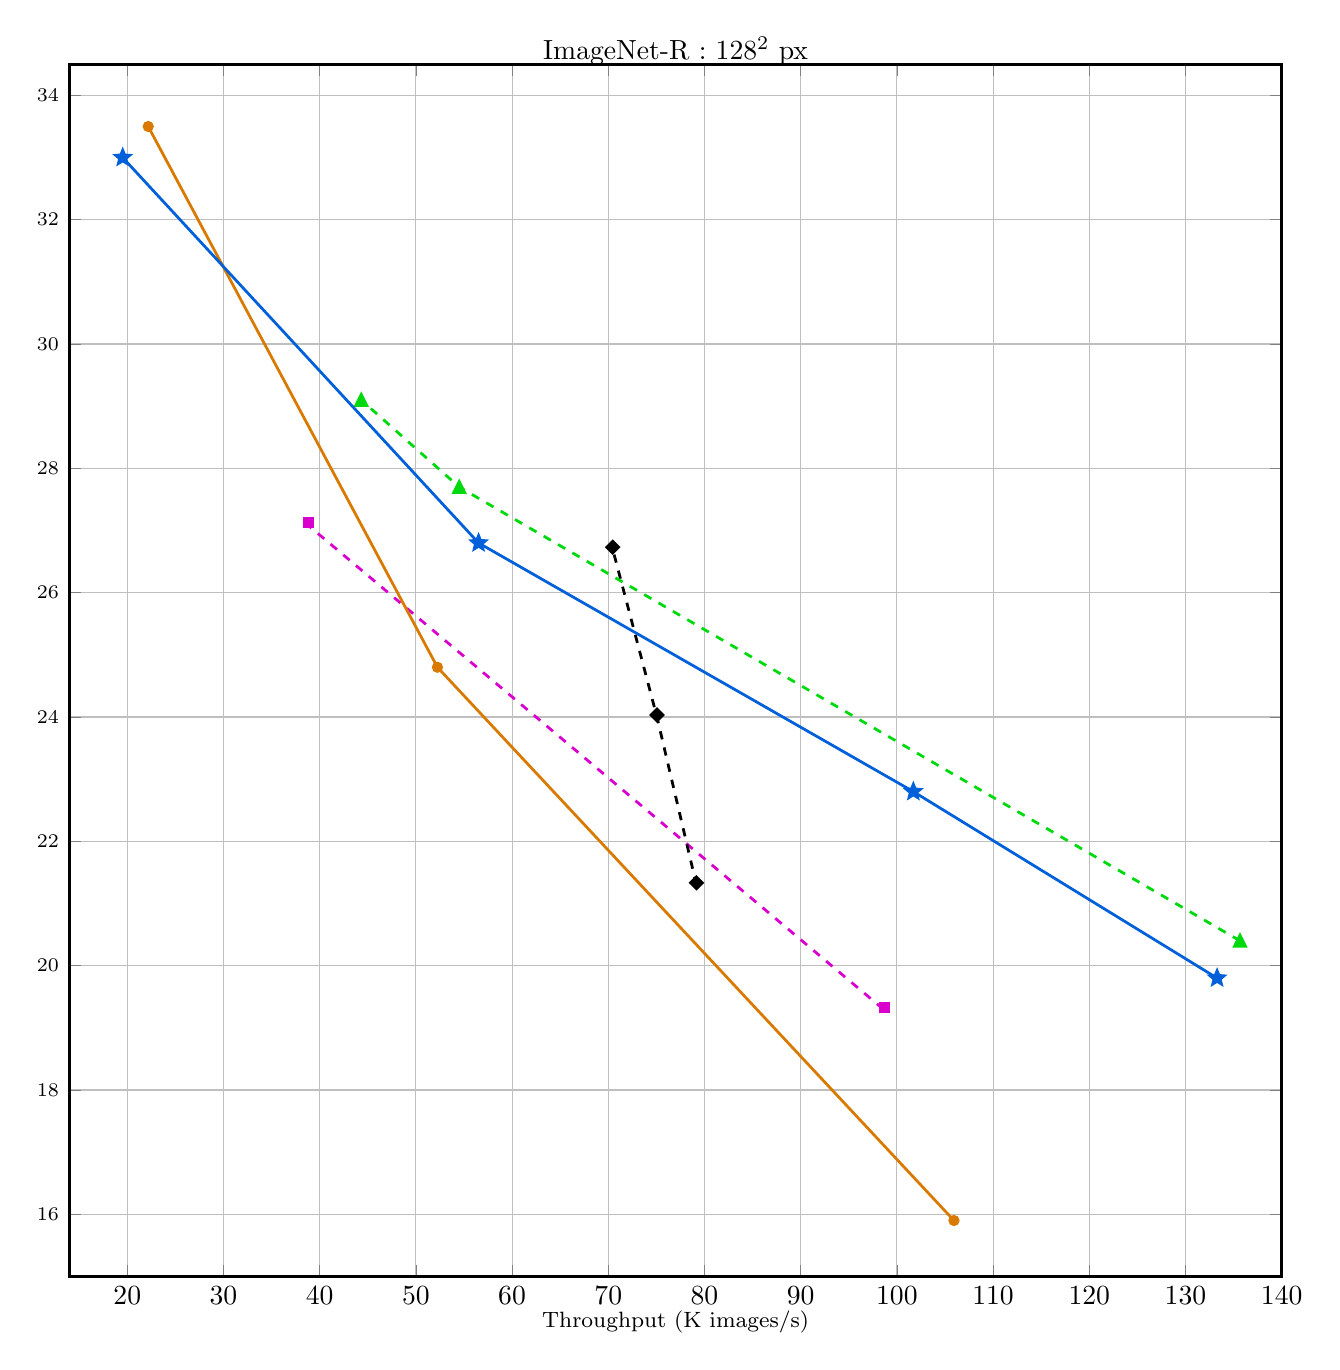
\begin{tikzpicture}
\begin{axis}[
    width=1.4\linewidth,
    height=1.4\linewidth,
    title={ImageNet-R : $128^2$ px},
    title style={yshift=-10pt},
    xlabel={Throughput (K images/s)},
    ylabel shift=-5pt,
    xlabel shift=-5pt,
    xmin=14, xmax=140,
    ymin=15, ymax=34.5,
    grid=major,
    line width=1pt,
    yticklabel style={font=\scriptsize},
    xlabel style={font=\footnotesize}
]
% \shade[
%     right color=yellow!60,
%     left color=white,
%     middle color=white,
%     samples=100,
%     opacity=0.2
% ] (rel axis cs:0,1) -- (rel axis cs:1,1) -- (rel axis cs:1,0) -- cycle;

% \shade[
%     top color=yellow!60,
%     bottom color=white,
%     middle color=white,
%     samples=100,
%     opacity=0.2
% ] (rel axis cs:0,1) -- (rel axis cs:1,1) -- (rel axis cs:1,0) -- cycle;

% \node[anchor=south west] at (rel axis cs:0.72,0.87) {\scriptsize optimal};
% ------------------------------------------------------
% 1) EFFICIENTVIT (ICCV 2023)
% ------------------------------------------------------
\draw[\efficientColor, line width=1pt, style=dashed]
  (axis cs:98.585, 19.3) coordinate (B1)
  -- (axis cs:38.683, 27.1) coordinate (B2);

\EfficientMarker[0.5]{(B1)}
\EfficientMarker[0.5]{(B2)}

% ------------------------------------------------------
% 2) SHVIT (CVPR 2024)
% ------------------------------------------------------
\draw[\shvitColor, line width=1pt, style=dashed]
  (axis cs:79.163, 21.3) coordinate (S1)
  -- (axis cs:75.060, 24.0) coordinate (S2)
  -- (axis cs:70.458, 26.7) coordinate (S3);

\ShvitMarker[0.5]{(S1)}
\ShvitMarker[0.5]{(S2)}
\ShvitMarker[0.5]{(S3)}

% ------------------------------------------------------
% 3) MOBILENETV4 (ECCV 2024)
% ------------------------------------------------------
\draw[\mobileColor, line width=1pt, style=dashed]
  (axis cs:135.663, 20.4) coordinate (M1)
  -- (axis cs:54.500, 27.7)  coordinate (M2)
  -- (axis cs:44.325, 29.1)  coordinate (M3);

\MobileMarker[1.0]{(M1)}
\MobileMarker[1.0]{(M2)}
\MobileMarker[1.0]{(M3)}

% ------------------------------------------------------
% 4) VIT+REGISTERS (ICLR 2024)
% ------------------------------------------------------
\draw[\registerColor, line width=1pt]
  (axis cs:105.933, 15.9) coordinate (R1)
  -- (axis cs:52.241, 24.8)  coordinate (R2)
  -- (axis cs:22.176, 33.5)  coordinate (R3);

\RegisterMarker[0.5]{(R1)}
\RegisterMarker[0.5]{(R2)}
\RegisterMarker[0.5]{(R3)}

% ------------------------------------------------------
% 5) VIT+JUMBO (ours)
% ------------------------------------------------------
\draw[\jumboColor, line width=1pt]
  (axis cs:133.285,19.8) coordinate (J0)
  -- (axis cs:101.711, 22.8) coordinate (J1)
  -- (axis cs:56.516,26.8) coordinate (J2)
  -- (axis cs:19.524,33.0) coordinate (J3);

\JumboMarker[0.25]{(J0)}
\JumboMarker[0.25]{(J1)}
\JumboMarker[0.25]{(J2)}
\JumboMarker[0.25]{(J3)}

\end{axis}
\end{tikzpicture}

        \phantomcaption
        \label{fig:sub:plot4}
    
    \end{subfigure}
    \vspace{-0.5cm}
    
    Legend: \InlineJumboMarker \hspace{0.01cm} ViT+Jumbo (ours),\hspace{0.2cm} \InlineRegisterMarker \hspace{0.01cm} ViT+Registers,\hspace{0.2cm} \InlineMobileMarker \hspace{0.01cm} MobileNetV4,\hspace{0.2cm} \InlineShvitMarker \hspace{0.01cm} SHViT,\hspace{0.2cm} \InlineEfficientMarker \hspace{0.01cm} EfficientViT

    \vspace{-0.2cm}
    \caption{ViT+Jumbo mostly achieves the Pareto frontier, while being much simpler than specialized compute-efficient model architectures. Results from each model's best learning rate is plotted. Throughput is measured on an RTX 4090 GPU using PyTorch 2.6.0, \texttt{torch.compile}, and a $512$ batch size.}
    \label{fig:1k_results}
    \vspace{-0.3cm}
\end{minipage}
\end{figure*}

\subsubsection{Experimental Details}\label{subsubsec:1k_setup}

\textbf{Setup.} We train models from scratch on ImageNet-1K \cite{russakovsky2015imagenet} using function matching \cite{beyer2022knowledge} with a highly accurate teacher ($85.7\%$ top-1 accuracy on ImageNet-1K \cite{touvron2022deit}) at $128\times128$ px for $400$ epochs. Then we finetune each model at $224\times224$ px for $20$ epochs with a more accurate (but expensive) teacher ($87.0\%$ top-1 accuracy on ImageNet-1K \cite{touvron2022deit}). Each run takes $4$-$5$ days on an RTX 4090 GPU.

This approach has three advantages. \circlednum{1} By training at two resolutions, we can compare the accuracy-speed trade-offs of models at two resolutions (rather than a single comparison point). \circlednum{2} By training at a lower resolution for the majority of epochs, we save \emph{significant} training cost, and models benefit from the FixRes effect \cite{touvron2019fixing, touvron2022deit}. \circlednum{3} By leveraging a SOTA distillation method, models benefit from greater sample efficiency. Importantly, both low-res to high-res training and function matching are \emph{architecture agnostic} --- they were invented with CNNs and are used with ViTs.

We train each model architecture twice, once for each learning rate \{$1$e$-3$, $3$e$-3$\} using a $1024$ batch size with the AdamW optimizer \cite{loshchilov2017decoupled}. We report the results of the best learning rate for each model architecture. Please see Appendix \ref{appendix:1K_hparams} for the complete results and hyperparameters.

\textbf{Baselines.} We choose the fastest models for each family: \circlednum{1} ViT+Registers \{nano, tiny, small\} \cite{darcet2024vision}, \circlednum{2} EfficientViT \{B0, B1\} \cite{cai2023efficientvit}, \circlednum{3} SHViT \{S1, S2, S3\} \cite{yun2024shvit}, and \circlednum{4} MobileNetV4 \{conv-small, conv-medium, hybrid-medium\} \cite{qin2025mobilenetv4}. We compare these architectures with our fastest ViT+Jumbo variants \{pico, nano, tiny, small\}. \citet{darcet2024vision} show ViT+Registers with $R$=$16$ performs best, which we confirm in Appendix \ref{appendix:reg} and use in these experiments. We show ViT+Jumbo is robust to the choice of $J$; we use $J$=$6$ and study its effect in subsection \ref{subsec:ablations}.

\textbf{Test Sets.} We test all models on the three most common ImageNet-1K test sets: ImageNet-Val \cite{russakovsky2015imagenet}, ImageNet-ReaL \cite{beyer2020we}, and ImageNet-v2 \cite{recht2019imagenet}. We also test all models on a newer, high-quality ImageNet-1K test set, ImageNet-HR \cite{fuller2024lookhere}, and an out-of-distribution test set, ImageNet-R \cite{hendrycks2021many}.

\subsubsection{High-Speed Results}

As illustrated in Fig \ref{fig:1k_results}, Jumbo mostly achieves the Pareto frontier among fast models on ImageNet-1K. We highlight the significance of these results, as Jumbo achieves them while preserving the many advantages and simplicity of plain ViTs; even matching the specialized compute-efficient architectures makes a strong case for ViT+Jumbo.

ViT+Jumbo outperforms ViT+Registers by $13.5\%$ at the nano scale and $3.2\%$ at the tiny scale, tested on $224 \times 224$ px images. These are \emph{significant} gains. And it confirms our first hypothesis that Jumbo's gains should increase as we decrease the patch width, i.e., from small ($D$=$384$) to tiny ($D$=$192$) to nano ($D$=$128$).

If a researcher or practitioner requires out-of-the-box support for SSL algorithms or multimodal processing, \emph{and} requires a fast model, ViT+Jumbo is a clear choice. ViT+Registers is not performant at high speeds, while the specialized compute-efficient architectures do not support most SOTA SSL algorithms or multimodal processing. Remote sensing \cite{pmlr-v235-rolf24a} and autonomous driving \cite{muhammad2020deep} are two of many applications where this combination of speed, SSL support, and multimodal processing is particularly valuable.

At the ViT-small scale (i.e., depth=$12$, width=$384$), ViT+Jumbo has \emph{no} gains over ViT+Registers ---  at least on ImageNet-1K. However, there is no fundamental reason to see gains generally stop at the ViT-small scale. It seems like a $384$-d \texttt{CLS} token can sufficiently model ImageNet-1K's output dimensionality. Furthermore, this singular negative result leads us to test our second hypothesis that Jumbo's gains should increase on tasks that require reasoning over a larger concept space.

\subsection{ImageNet-21K Experiments}\label{subsec:21k}

ImageNet-1K is a subset of the more challenging, original ImageNet \cite{deng2009imagenet}, now commonly referred to as ImageNet-21K. We use a common variant comprising $10450$ classes; this is a processed variant intended to make training on ImageNet-21K more accessible \cite{ridnik2021imagenetk} (they call this variant ImageNet-21K-P, but we refer to it as ImageNet-21K). This dataset provides more than $\times 10$ the number of classes and samples as ImageNet-1K --- making it well suited to test our second hypothesis.

\subsubsection{Experimental Details}

\textbf{Setup.} We train models from scratch on ImageNet-21K \cite{ridnik2021imagenetk}. Since training models on ImageNet-21K is expensive, we leverage a token dropping strategy to reduce costs. Specifically, we start training with a $90$\% token drop rate and linearly decrease this value to $10$\%; this halves the total number of tokens processed. \citet{dehghani2024patch} demonstrate the effectiveness of this strategy, i.e., leveraging ``masking'' with plain supervised training. Moreover, all the models that we train on ImageNet-21K support token dropping with minimal code changes. 

We train each model architecture once, for $50$ epochs using a $3$e$-3$ learning rate and a $1024$ batch size with the AdamW optimizer \cite{loshchilov2017decoupled} (see Appendix \ref{appendix:1K_hparams} for other hyperparameters). Each ViT-base run takes $7$ days, and each ViT-small run takes $3.3$ days on an RTX 4090 GPU.

\textbf{Baselines.} We choose ViT+Registers \{small, base\} to compare with our ViT+Jumbo \{small, base\} sizes. This is a more narrow but valid comparison, as the plain ViT is the vision community's preferred architecture at these scales --- due to its simplicity, flexibility, and out-of-the-box compatibility with SSL algorithms. For ViT+Registers, we use $R$=$16$; for ViT+Jumbo, we use $J$=$6$ for the small model (since it worked well on ImageNet-1K) and $J$=$3$ for the base model (since $J$=$6$ did not fit in memory; we discuss and demonstrate a solution to this limitation in section \ref{sec:discussion}).

\subsubsection{ImageNet-21K Results}

ViT+Jumbo outperforms ViT+Registers by $3.4\%$ and $1.0\%$ at ViT-small and ViT-base scales, respectively (see Fig. \ref{fig:sub:21k}). These significant gains confirm our second hypothesis that Jumbo's gains should increase with increasing output dimensionality. Since Jumbo scales favorably with output dimensionality, we expect Jumbo to excel at CLIP-like \cite{radford2021learning} vision-language frameworks, where the ViT is tasked with modeling a vocabulary with $50$K+ terms. However, these experiments require even more resources, so we save them for future work.

\subsection{Time Series Experiments}\label{subsec:time}
Users can easily adapt Jumbo to different input shapes, i.e., beyond images. This subsection demonstrates one such adaptation to time series inputs.

PatchTST \cite{Yuqietal-2023-PatchTST} is a SOTA patch-based transformer architecture for time series processing, designed to address the limited semantic meaning carried by individual points in time. We extend PatchTST by introducing registers to its transformer backbone (PatchTST+Registers) and incorporating Jumbo (PatchTST+Jumbo).

\subsubsection{Experimental Details}

\textbf{Setup.} We train models from scratch on \circlednum{1} $10$ univariate time series datasets from the UCR archive \cite{UCRArchive}, and \circlednum{2} $10$ multivariate time series datasets from the UEA archive \cite{UEAArchive}; both of which are commonly used benchmarks  \cite{ZerveasTST, S3TimeSeries, ShapeFormer}. 
For each dataset and model architecture, we perform a hyperparameter sweep that is the result of the following Cartesian product: learning rate \{$3$e$-3$, $1$e$-3$, $3$e$-4$, $1$e$-4$\}, and dropout \{$0.0$, $0.1$, $0.2$\}. 
Additional hyperparameter and training details are provided in Appendix \ref{appendix:TST_hyperparameters}, where we also report both the best run and the average of all $12$ runs per dataset and architecture.
To summarize these many results, we compute the rank between models, then average the ranks over the $10$ univariate and $10$ multivariate datasets.

\textbf{Baselines.}
We compare PatchTST with our PatchTST+Jumbo models and create PatchTST+Registers as an additional baseline.
We experiment with $8$ and $42$ patches per sequence for all three architectures.
Importantly, adding our Jumbo \texttt{CLS} token or registers to the PatchTST architecture is simple to adopt.

\subsubsection{Time Series Results}

% \usepackage{booktabs}


\begin{table}
	\centering
	\caption{Analysis of models' inference speed.}
	\begin{tabular}{c|ccc} 
		\toprule
		& Parms (MB) & Speed & Moderate  \\ 
		\hline
		IA-SSD     & 2.7        & 84    & 79.12     \\
		PDM-SSD(A) & 3.3        & 84    & 79.37     \\
		PDM-SSD(J) & 3.3        & 68    & 79.75     \\
		\bottomrule
	\end{tabular}
\label{tabel8}
\end{table}

Our extensive evaluations demonstrate that PatchTST+Jumbo outperforms strong PatchTST and PatchTST+Registers baselines (Tab. \ref{tab:timeseries}).
In particular, Jumbo gains the most with fewer patches and when results are averaged across all runs.
These results demonstrate Jumbo's potential in applications that leverage plain, noncausal transformers.
% As the broader science and engineering community continues to apply transformers, the number of these applications grows, so retaining compatibility with plain transformers enables more general usage.
As transformers are increasingly adopted in a wide variety of important science and engineering challenges, improving plain transformers (rather than application-specific niche improvements) will achieve broader impact.

\subsection{Ablations}\label{subsec:ablations}

\begin{table}[!th]\centering\scriptsize
    \caption{Jumbo multiplier $J$ and inner Jumbo FFN multiplier ablations. Throughput measurements and evaluations are performed on $128\times128$ px images. Our default values are in gray.}
    \label{tab:combined_ablation}
    \setlength{\tabcolsep}{2pt}
        \begin{tabular}{
            c
            c
            c
            c
            c
        }   \toprule
            \makecell{Patch\\Width} &
            \makecell{Jumbo\\Multiplier} &
            \makecell{Inner FFN\\Multiplier} &
            \makecell{Throughput\\imgs/s} &
            \makecell{ImageNet-Val\\\% Top-1 Acc.}\\
            \toprule
            \multirow{8}{*}{192} & \multirow{2}{*}{2} & 2 & 71.6K & 70.0\\
            & & 4 & 69.6K & 70.4\\
            \noalign{\vskip -0.25em}\cmidrule{2-2}\noalign{\vskip -0.25em}
            & \multirow{3}{*}{4} & 1 & 69.6K & 71.5\\
            & & 2 & 68.1K & 70.6\\
            & & 4 & 64.9K & 72.2\\
            \noalign{\vskip -0.25em}\cmidrule{2-2}\noalign{\vskip -0.25em}
            & \multirow{3}{*}{6} & 1 & 65.3K & 72.1\\
            & & 2 & 63.5K & 71.8\\
            & & \graycell{4} & \graycell{56.5K} & \graycell{73.0}\\
            \midrule
            \multirow{8}{*}{384} & \multirow{2}{*}{2} & 2 & 27.2K & 77.0\\
            & & 4 & 26.1K & 78.1\\
            \noalign{\vskip -0.25em}\cmidrule{2-2}\noalign{\vskip -0.25em}
            & \multirow{3}{*}{4} & 1 & 26.1K & 77.3\\
            & & 2 & 24.5K & 77.9\\
            & & 4 & 23.6K & 77.9\\
            \noalign{\vskip -0.25em}\cmidrule{2-2}\noalign{\vskip -0.25em}
            & \multirow{3}{*}{6} & 1 & 23.9K & 77.6\\
            & & 2 & 22.9K & 77.8\\
            & & \graycell{4} & \graycell{19.5K} & \graycell{78.3}\\
            \bottomrule
        \end{tabular}
\end{table}

\textbf{Setup.} We follow our ImageNet-1K training recipe, training models using function matching \cite{beyer2022knowledge}, for $400$ epochs at $128\times128$ px. We vary the Jumbo multiplier, $J$, and the inner Jumbo FFN multiplier; this inner multiplier increases the hidden size of the Jumbo FFN, and we always use the default value of $4$ for patches. We test models at $128\times128$ px.

\textbf{Results.} 
Our method is robust to the choice of Jumbo multiplier and inner Jumbo FFN multiplier (Tab. \ref{tab:combined_ablation}), although generally, higher multipliers perform better on ImageNet-1K.
For simplicity, we use the largest multipliers as the defaults (gray) and use them in our apples-to-apples comparisons (i.e., subsections \ref{subsec:1k} and \ref{subsec:21k}).
However, lower values may provide slightly better accuracy-speed trade-offs. Please see Appendix \ref{appendix:ablations} for complete results.

\section{Discussion}\label{sec:discussion}

\begin{table}[t]
    \centering
    \scriptsize
    \caption{We limit Jumbo's parameter increase by sharing Jumbo weights across layers. Separately, we let the Jumbo layers differ via layer-specific LoRAs \cite{hu2022lora}. Both methods effectively control Jumbo's parameter increase while maintaining strong performance. We measure throughput/memory on an RTX 4090 GPU with a $512$ batch size; we train and test models on ImageNet-21K.}
    \setlength{\tabcolsep}{2pt}
    \begin{tabular}{lcccc} 
        \toprule
        Architecture & \makecell{Throughput\\imgs/s} & \makecell{Params\\M} & \makecell{Memory\\GB} & \makecell{Top-1 Acc.\\$\%$} \\
         \midrule
            ViT+Registers, $R$=$16$ & 8.4K & 25.7 & 3.47 & 41.48 \\
            ViT+Jumbo, $J$=$6$ & 8.0K & 555.6 & 5.39 & 44.95 \\
            ViT+Jumbo, layer share, $J$=$6$ & 8.2K & 88.3 & 3.76 & 44.61 \\
            ViT+Jumbo+LoRA, $J$=$6$, rank=$8$ & 8.1K & 88.8 & 3.95 & 44.94 \\
            ViT+Jumbo+LoRA, $J$=$6$, rank=$32$ & 8.1K & 90.1 & 3.64 & 44.97 \\
         \bottomrule
    \end{tabular}
    \label{tab:bonus}
\end{table}

\textbf{Limitations.} Jumbo's most significant limitation is the parameter increase due to dedicating a separate FFN to the Jumbo \texttt{CLS} token (instead of sharing parameters between patches) and increasing the size of this Jumbo FFN.
For \emph{many} applications, increasing speed is more helpful than increasing memory is harmful.
For memory-constrained applications, we propose a solution to control this cost: tie Jumbo's FFN parameters across layers.
This strategy results in a $12\times$ reduction in additional model parameters (our models have $12$ layers).
We also experiment with applying layer-specific LoRAs \cite{hu2022lora} to the tied Jumbo parameters; this is a parameter-efficient means of enabling the Jumbo FFNs to differ across layers and is similar to \citet{li2024lors}.
We find that both methods are highly effective at controlling Jumbo's parameter count (Tab. \ref{tab:bonus}).

\textbf{Conclusion.}
Jumbo is a highly promising and elegantly simple method that increases the global reasoning capacity of plain ViTs while maintaining throughput.
Jumbo is most helpful when the patch token width is otherwise too narrow for the task; we demonstrate this by decreasing the patch token width and, separately, increasing the output dimensionality.
There are many exciting ways to apply Jumbo, such as zero-shot image classification, which can have large output vocabularies that we expect Jumbo to better model.
There are also many ways to extend Jumbo, for example, by including multiple shared Jumbo tokens (e.g., two shared $J$=$2$ Jumbo tokens) or parameter-efficient alternatives to dense linear layers to control memory costs further \cite{qiu2024compute}.

\clearpage

\section*{Impact Statement}
This work presents new designs and empirical results for deep network architectures for more accurate and computationally efficient modeling applied to visual recognition and time series processing.
This general topic does not have more specific societal consequences aside from those inherited, good or bad, from the adoption of machine learning.

\bibliography{example_paper}
\bibliographystyle{icml2025}


%%%%%%%%%%%%%%%%%%%%%%%%%%%%%%%%%%%%%%%%%%%%%%%%%%%%%%%%%%%%%%%%%%%%%%%%%%%%%%%
%%%%%%%%%%%%%%%%%%%%%%%%%%%%%%%%%%%%%%%%%%%%%%%%%%%%%%%%%%%%%%%%%%%%%%%%%%%%%%%
% APPENDIX
%%%%%%%%%%%%%%%%%%%%%%%%%%%%%%%%%%%%%%%%%%%%%%%%%%%%%%%%%%%%%%%%%%%%%%%%%%%%%%%
%%%%%%%%%%%%%%%%%%%%%%%%%%%%%%%%%%%%%%%%%%%%%%%%%%%%%%%%%%%%%%%%%%%%%%%%%%%%%%%
\newpage
\appendix
\onecolumn
\section{Appendix}

\subsection{Compute-efficient Architecture Descriptions}\label{appendix:related_work}

\circlednum{1} EfficientViT \cite{cai2023efficientvit} is a hierarchical architecture with four stages and one head. Stages $1$ and $2$ consist of MBConv layers \cite{sandler2018mobilenetv2}. Stages $3$ and $4$ consist of MBConv sublayers and their novel EfficientViT sublayer, consisting of an efficient attention module and an FFN+DWConv module \cite{howard2017mobilenets}. Their attention module creates queries, keys, and values of three scales via three DWConvs, and then each set of queries, keys, and values undergoes efficient linear attention. Finally, the head receives outputs from Stages $2$, $3$, and $4$, and applies a final MBConv. EfficientViT variants differ in stage depths and widths, as well as head width.

\circlednum{2} SHViT \cite{yun2024shvit} is a hierarchical architecture with three stages. Stage $1$ consists of a DWConv+BatchNorm sublayer and an FFN sublayer. Stages $2$ and $3$ incorporate their novel single-headed self-attention (SHSA) sublayer between the stage $1$ sublayers. SHSA consists of performing single-headed self-attention on a fraction of dimensions ($1/4.67$ ratio); the other dimensions pass straight through, further reducing cost. Both FFN and SHSA sublayers also replace linear layers with DWConv. SHViT variants differ in stage depths and widths.

\circlednum{3} MobileNetV4 \cite{qin2025mobilenetv4} variants use their FusedIB, ExtraDW, and Mobile MQA (multi-query attention) modules along with MBConv, ConvNext-Like \cite{liu2022convnet}, and FFN modules. Variants differ in stage depths and widths, the number of stages, and stage architectures built with a combination of the listed modules.

\subsection{Experimental Details}\label{appendix:experimental_details}

\subsubsection{ImageNet-1K and -21K Hyperparameters}\label{appendix:1K_hparams}
We pick these recipes based on findings in the literature --- such as \citet{touvron2022deit}, \citet{fuller2024lookhere}, \citet{beyer2022knowledge}, \citet{dehghani2024patch}, and \citet{steiner2022how} --- and past experience indicating that these recipes would result in strong models.

\textbf{ImageNet-1K training recipe:} $128\times 128$ px images, $400$ epochs, $1024$ batch size, PyTorch's AdamW optimizer with a $0.05$ weight decay, $1.0$ clip grad norm, \texttt{deit3-base-patch16-224.fb-in22k-ft-in1k} teacher \cite{touvron2022deit} given $224\times224$ px images using \citet{rw2019timm}'s implementation, KL divergence loss between student and teacher logits \cite{beyer2022knowledge}, linear learning rate warmup for $10\%$ of steps to $\{1$e$-3, 3$e$-3\}$ and cooldown using a cosine decay schedule to $1$e$-5$, mixup $\alpha=0.8$, cutmix $\alpha=1$, and 3-Augment data augmentation \cite{touvron2022deit}.

\textbf{ImageNet-1K finetuning recipe:} $224\times 224$ px images, $20$ epochs, $512$ batch size, PyTorch's AdamW optimizer with a $0.1$ weight decay, $1.0$ clip grad norm, \texttt{deit3-large-patch16-224.fb-in22k-ft-in1k} teacher \cite{touvron2022deit} given $224\times224$ px images using \citet{rw2019timm}'s implementation, KL divergence loss between student and teacher logits \cite{beyer2022knowledge}, linear learning rate warmup for $25\%$ of steps to $5$e$-5$ and cooldown using a cosine decay schedule to $1$e$-5$, mixup $\alpha=0.8$, cutmix $\alpha=1$, and AutoAugment (``rand-m9-mstd0.5-inc1'') data augmentation \cite{cubuk2018autoaugment} following DEIT III's \cite{touvron2022deit} high-res finetuning recipe.

\textbf{ImageNet-21K training recipe:} $224\times 224$ px images, $50$ epochs, $1024$ batch size, PyTorch's AdamW optimizer with a $0.02$ weight decay, $1.0$ clip grad norm, cross-entropy loss, linear learning rate warmup for $10\%$ of steps to $3$e$-3$ and cooldown using a cosine decay schedule to $1$e$-5$, mixup $\alpha=0.8$, cutmix $\alpha=0$, and 3-Augment data augmentation \cite{touvron2022deit}. To speed up training, we also employ a token dropping strategy starting at $90\%$, linearly decreasing to $10\%$.

\subsubsection{Time Series Experiments}\label{appendix:TST_hyperparameters}
We adopt the PatchTST \cite{Yuqietal-2023-PatchTST} architecture for our time series experiments. PatchTST is a patch-based transformer architecture for time series processing. The method splits a univariate time series into patches processed as they are in ViTs for classification, aside from position encoding ($2$D vs. $1$D). For multivariate series, each channel is processed \textit{independently} using the shared transformer backbone, with the final-layer \texttt{CLS} tokens from each channel concatenated before classification. We extend this shared backbone with registers (PatchTST+Registers) and Jumbo (PatchTST+Jumbo).

We closely follow the PatchTST training recipe for our experiments, making minor adjustments based on prior experience to enhance performance. This method remains competitive with recent transformer-based benchmarks for time series classification \cite{ZerveasTST, S3TimeSeries, ShapeFormer}. Apart from variations in time series length, all experiments use the same hyperparameters and methodology.

\textbf{PatchTST Hyperparameters:} The model comprises $3$ encoder layers, each with $16$ attention heads and a token width of $D = 128$. The transformer FFN includes two linear layers with a GELU activation \cite{gelu}; the first expands the hidden dimension to $256$, while the second projects it back to $128$. For PatchTST+Jumbo, we use $J=4$. For PatchTST+Registers, $R$ is calculated according to Appendix \ref{appendix:flop_details}.

\textbf{Time Series training recipe:}
We perform a hyperparameter sweep over the Cartesian product of learning rates \{$3$e$-3$, $1$e$-3$, $3$e$-4$, $1$e$-4$\} and dropout rates \{$0.0$, $0.1$, $0.2$\}. Each configuration uses either $8$ or $42$ equally sized patches of maximum possible length, with end-padding applied as needed. The stride length is set to half the patch length. Unless stated otherwise, all experiments follow the same setup: $100$ epochs, $256$ batch size, PyTorch’s AdamW optimizer with a $0.02$ weight decay, cross-entropy loss, and a linear learning rate warmup for the first $10\%$ of steps, followed by a cooldown using cosine decay to $1$e$-8$. For large datasets, we reduce the number of epochs to ensure efficient processing within a reasonable time frame; specifically, we train datasets $\{$Sleep$,~$Tiselac$,~ $FaceDetection$\}$ for $20$ epochs. 

Each dataset from the UEA and UCR archives includes a prescribed validation set. We create a new $50$/$50$ test/validation split from each of these original validation sets, selecting the best run based on validation performance. All reported results are from the \emph{test} set. 

The $20$ datasets were selected in decreasing order of their number of training examples; datasets with either (i) fewer than 42 total timesteps or (ii) significant data preparation issues were excluded.

\subsubsection{FLOP Details}\label{appendix:flop_details}

To ensure a fair comparison, we configure PatchTST+Registers and PatchTST+Jumbo to have approximately equal per-layer FLOPs by selecting the number of registers $R$ in the former and the Jumbo multiplier $J$ in the latter accordingly. Additionally, we apply average pooling to the $J$ split segments of the Jumbo token to prevent a significant increase in the number of learnable parameters of the classification head. This pooling produces a token of width $D$ per channel before concatenation, effectively serving the same role as a \texttt{CLS} token. The detailed per-layer FLOP calculation is provided by the propositon below.

\newtheorem{prop}{Proposition}

\begin{prop}
Let $P$ be the total number of local patch tokens, $R$ the number of register tokens, $D$ the width, and $J$ the Jumbo multiplier. Given an FFN hidden dimension of $2D$, and otherwise fixed parameters, a Register architecture with $R$ registers has the same per-layer FLOP count as a Jumbo architecture with multiplier $J$ if and only if
\[
    R = -(2D + P) + \sqrt{(2D + P)^2 + (1 + 2D)J^2 + 2(D + P)J}
\]
\end{prop}

\begin{proof}
Let $F$ denote the FLOP count. Given a sequence length of $n$ tokens, each of width $d$, the FLOP contributions from the MHSA and FFN sublayers in a single transformer layer with a FFN hidden dimension of $ld$ are given by
\[
    F_\text{MHSA} = 4nd^2 + 2n^2d
    ~~\text{and}~~
    F_{\text{FFN}} = l^2nd^2 = 4nd^2
\]
where we fix $l = 2$. For the Register architecture, $n = P + R$ and $d = D$ for both the MHSA and the FFN contributions. For the Jumbo architecture, $n = P + J$ and $d = D$ for MHSA. The FFN contribution is split; local patch tokens contribute with $n = P, d = D$ while the dedicated Jumbo FFN has $n = 1, d = JD$. From summing the contributions, it follows that 
\[
    \begin{split}
        F_\text{Reg} = 4(P + R)D^2 + 2(P + R)^2D + 4(P + R)D^2
        \\
        F_\text{Jumbo} = 4(P + R)D^2 + 2(P + R)D^2 + 4PD^2 + 4J^2D^2
    \end{split}
\]
Equating $F_\text{Reg} = F_\text{Jumbo}$ and solving for $R$ gives the stated result.
\end{proof}

In our time series experiments, we compute $R$, rounding to the nearest integer, to match the per-layer FLOP count of a Jumbo architecture with multiplier $J$ as closely as possible.

1. Distilling accelerated residuals from slow residuals
2. only one of them active -> either vla or m2r2\label{appendix:ablations}

\clearpage

\begin{table*}[!th]\centering\footnotesize
    \caption{ViT+Registers results, obtained on $128\times128$ px images ($\%$).}
    \label{tab:all_registers}
    \setlength{\tabcolsep}{2pt}
        \begin{tabular}{
            c
            c
            c
            c
            cc
            cc
            cc
            cc
            cc
        }   \toprule
            Patch & Num. & Learning & Throughput &
            \multicolumn{2}{c}{ImageNet-Val} & 
            \multicolumn{2}{c}{ImageNet-ReaL} & 
            \multicolumn{2}{c}{ImageNet-v2} & 
            \multicolumn{2}{c}{ImageNet-R} &
            \multicolumn{2}{c}{ImageNet-HR} \\
            Width & Registers & Rate & imgs/s &
            Top-1 & Top-5 & Top-1 & Top-5 & Top-1 & Top-5 & Top-1 & Top-5 & Top-1 & Top-5 \\
            \toprule
            \multirow{2}{*}{128} & \graycell{16} & \graycell{$3$e$-3$} & \multirow{2}{*}{105.9K} & \graycell{53.6}&	\graycell{78.5}&	\graycell{60.8}&	\graycell{83.6}&	\graycell{42.4}&	\graycell{67.8}&	\graycell{15.9}&	\graycell{28.6}&	\graycell{61.9}&	\graycell{83.4}\\
            & 16 & $1$e$-3$ & & 51.9&	76.8&	59.0&	81.8&	40.8&	65.4&	13.7&	24.9&	60.5&	82.6\\
            \midrule
            \multirow{3}{*}{192} & 8 & $3$e$-3$ & 59.9K & 68.5&	88.8&	76.1&	92.6&	55.7&	78.8&	24.9&	39.4&	77.8&	92.2\\
            & \graycell{16} & \graycell{$3$e$-3$} & \multirow{2}{*}{52.2K} & \graycell{68.8}&	\graycell{88.9}&	\graycell{76.6}&	\graycell{92.6}&	\graycell{55.9}&	\graycell{79.4}&	\graycell{24.8}&	\graycell{38.9}&	\graycell{78.5}&	\graycell{92.5}\\
            & 16 & $1$e$-3$ & & 66.1&	87.2&	74.0&	91.2&	54.2&	77.0&	22.9&	36.2&	75.4&	91.6\\
            \midrule
            \multirow{3}{*}{384} & 8 & $3$e$-3$ & 24.4K & 77.8&	93.9&	84.3&	96.2&	65.8&	86.3&	33.3&	48.6&	86.8&	96.5\\
            & 16 & $3$e$-3$ & \multirow{2}{*}{22.2K} & 78.1&	94.0&	84.5&	96.3&	66.1&	86.6&	33.3&	48.6&	86.6&	96.5\\
            & \graycell{16} & \graycell{$1$e$-3$} & & \graycell{78.2}&	\graycell{94.1}&	\graycell{84.5}&	\graycell{96.3}&	\graycell{66.4}&	\graycell{86.6}&	\graycell{33.5}&	\graycell{48.4}&	\graycell{87.2}&	\graycell{96.6}\\
            \bottomrule
        \end{tabular}
\end{table*}\label{appendix:reg}
\begin{table*}[!th]\centering\footnotesize
    \caption{ViT+Jumbo results, obtained on $128\times128$ px images ($\%$).}
    \label{tab:all_jumbo}
    \setlength{\tabcolsep}{2pt}
        \begin{tabular}{
            c
            c
            c
            cc
            cc
            cc
            cc
            cc
        }   \toprule
            Patch & Learning & Throughput &
            \multicolumn{2}{c}{ImageNet-Val} & 
            \multicolumn{2}{c}{ImageNet-ReaL} & 
            \multicolumn{2}{c}{ImageNet-v2} & 
            \multicolumn{2}{c}{ImageNet-R} &
            \multicolumn{2}{c}{ImageNet-HR} \\
            Width & Rate & imgs/s &
            Top-1 & Top-5 & Top-1 & Top-5 & Top-1 & Top-5 & Top-1 & Top-5 & Top-1 & Top-5 \\
            \toprule
            \multirow{2}{*}{96} & \graycell{$3$e$-3$} & \multirow{2}{*}{133.3K} & \graycell{64.0}&	\graycell{84.9}&	\graycell{71.2}&	\graycell{88.8}&	\graycell{50.6}&	\graycell{74.0}&	\graycell{19.8}&	\graycell{32.7}&	\graycell{72.7}&	\graycell{89.5}\\
            & $1$e$-3$ & & 63.2&	84.5&	70.3&	88.5&	49.8&	72.9&	18.7&	31.1&	72.0&	88.8\\
            \midrule
            \multirow{2}{*}{128} & $3$e$-3$ & \multirow{2}{*}{101.7K} & 68.2&	87.7&	75.2&	91.3&	55.0&	77.4&	23.2&	36.7&	77.3&	92.1\\
            & \graycell{$1$e$-3$} & & \graycell{68.8}&	\graycell{88.1}&	\graycell{75.6}&	\graycell{91.5}&	\graycell{55.1}&	\graycell{77.5}&	\graycell{22.8}&	\graycell{36.5}&	\graycell{77.9}&	\graycell{92.0}\\
            \midrule
            \multirow{2}{*}{192} & \graycell{$3$e$-3$} & \multirow{2}{*}{56.5K} & \graycell{73.0}&	\graycell{90.7}&	\graycell{79.6}&	\graycell{93.7}&	\graycell{59.4}&	\graycell{81.2}&	\graycell{26.8}&	\graycell{41.3}&	\graycell{82.3}&	\graycell{93.9}\\
            & $1$e$-3$ & & 72.6&	90.6&	79.2&	93.5&	58.8&	80.5&	25.7&	39.8&	81.6&	94.1\\
            \midrule
            \multirow{2}{*}{384} & $3$e$-3$ & \multirow{2}{*}{19.5K} & 78.3&	93.8&	84.2&	96.1&	66.1&	86.0&	32.9&	48.6&	87.0&	96.3\\
            & \graycell{$1$e$-3$} & & \graycell{78.5}&	\graycell{94.2}&	\graycell{84.4}&	\graycell{96.3}&	\graycell{65.8}&	\graycell{86.4}&	\graycell{33.0}&	\graycell{48.7}&	\graycell{87.2}&	\graycell{96.3}\\
            \bottomrule
        \end{tabular}
\end{table*}
\begin{table*}[!th]\centering\footnotesize
    \caption{MobileNetV4 results, obtained on $128\times128$ px images ($\%$).}
    \label{tab:all_mobilenet}
    \setlength{\tabcolsep}{2pt}
        \begin{tabular}{
            c
            c
            c
            cc
            cc
            cc
            cc
            cc
        }   \toprule
            \multirow{2}{*}{Size} & Learning & Throughput &
            \multicolumn{2}{c}{ImageNet-Val} & 
            \multicolumn{2}{c}{ImageNet-ReaL} & 
            \multicolumn{2}{c}{ImageNet-v2} & 
            \multicolumn{2}{c}{ImageNet-R} &
            \multicolumn{2}{c}{ImageNet-HR} \\
             & Rate & imgs/s &
            Top-1 & Top-5 & Top-1 & Top-5 & Top-1 & Top-5 & Top-1 & Top-5 & Top-1 & Top-5 \\
            \toprule
            \multirow{2}{*}{conv-small} & \graycell{$3$e$-3$} & \multirow{2}{*}{135.7K} & \graycell{62.1}&	\graycell{83.6}&	\graycell{69.2}&	\graycell{88.1}&	\graycell{49.1}&	\graycell{72.8}&	\graycell{20.4}&	\graycell{34.3}&	\graycell{71.8}&	\graycell{89.4}\\
             & $1$e$-3$ &  & 60.0&	82.0&	67.2&	86.7&	47.6&	71.4&	18.9&	32.2&	69.8&	87.7\\
            \midrule
            \multirow{2}{*}{conv-medium} & \graycell{$3$e$-3$} & \multirow{2}{*}{54.5K} & \graycell{73.3}&	\graycell{91.5}&	\graycell{80.5}&	\graycell{94.6}&	\graycell{60.6}&	\graycell{82.9}&	\graycell{27.7}&	\graycell{42.8}&	\graycell{83.2}&	\graycell{95.3}\\
             & $1$e$-3$ & & 72.2&	90.7&	79.4&	94.0&	59.5&	81.7&	27.0&	42.0&	82.0&	94.6\\
            \midrule
            \multirow{2}{*}{hybrid-medium} & $3$e$-3$ & \multirow{2}{*}{44.3K} & 74.9&	92.4&	81.8&	95.3&	62.4&	84.0&	29.5&	44.8&	84.4&	95.5\\
             & \graycell{$1$e$-3$} & & \graycell{75.2}&	\graycell{92.5}&	\graycell{82.0}&	\graycell{95.3}&	\graycell{63.0}&	\graycell{84.5}&	\graycell{29.1}&	\graycell{44.5}&	\graycell{84.2}&	\graycell{95.4}\\
            \bottomrule
        \end{tabular}
\end{table*}
\begin{table*}[!th]\centering\footnotesize
    \caption{SHViT results, obtained on $128\times128$ px images ($\%$).}
    \label{tab:all_shvit}
    \setlength{\tabcolsep}{2pt}
        \begin{tabular}{
            c
            c
            c
            cc
            cc
            cc
            cc
            cc
        }   \toprule
            \multirow{2}{*}{Size} & Learning & Throughput &
            \multicolumn{2}{c}{ImageNet-Val} & 
            \multicolumn{2}{c}{ImageNet-ReaL} & 
            \multicolumn{2}{c}{ImageNet-v2} & 
            \multicolumn{2}{c}{ImageNet-R} &
            \multicolumn{2}{c}{ImageNet-HR} \\
             & Rate & imgs/s &
            Top-1 & Top-5 & Top-1 & Top-5 & Top-1 & Top-5 & Top-1 & Top-5 & Top-1 & Top-5 \\
            \toprule
            \multirow{2}{*}{S1} & $3$e$-3$ & \multirow{2}{*}{79.2K} & 63.5&	84.9&	70.9&	89.1&	50.8&	74.5&	22.2&	35.7&	73.7&	90.0\\
             & \graycell{$1$e$-3$} &  & \graycell{63.5}&	\graycell{85.1}&	\graycell{71.0}&	\graycell{89.3}&	\graycell{50.9}&	\graycell{74.4}&	\graycell{21.3}&	\graycell{34.7}&	\graycell{72.9}&	\graycell{90.5}\\
            \midrule
            \multirow{2}{*}{S1} & $3$e$-3$ & \multirow{2}{*}{75.1K} & 66.6&	87.0&	73.9&	90.8&	54.0&	76.6&	23.9&	38.0&	76.1&	91.7\\
             & \graycell{$1$e$-3$} & & \graycell{66.7}&	\graycell{87.0}&	\graycell{73.8}&	\graycell{90.8}&	\graycell{53.7}&	\graycell{76.8}&	\graycell{24.0}&	\graycell{37.8}&	\graycell{76.7}&	\graycell{92.0}\\
            \midrule
            \multirow{2}{*}{S3} & $3$e$-3$ & \multirow{2}{*}{70.4K} & 70.5&	89.8&	77.7&	93.1&	58.1&	80.4&	26.6&	41.0&	80.4&	93.8\\
            & \graycell{$1$e$-3$} & & \graycell{71.2}&	\graycell{90.0}&	\graycell{78.3}&	\graycell{93.3}&	\graycell{58.6}&	\graycell{80.7}&	\graycell{26.7}&	\graycell{40.7}&	\graycell{80.7}&	\graycell{93.9}\\
            \bottomrule
        \end{tabular}
\end{table*}
\begin{table*}[!th]\centering\footnotesize
    \caption{EfficientViT results, obtained on $128\times128$ px images ($\%$).}
    \label{tab:all_efficientvit}
    \setlength{\tabcolsep}{2pt}
        \begin{tabular}{
            c
            c
            c
            cc
            cc
            cc
            cc
            cc
        }   \toprule
            \multirow{2}{*}{Size} & Learning & Throughput &
            \multicolumn{2}{c}{ImageNet-Val} & 
            \multicolumn{2}{c}{ImageNet-ReaL} & 
            \multicolumn{2}{c}{ImageNet-v2} & 
            \multicolumn{2}{c}{ImageNet-R} &
            \multicolumn{2}{c}{ImageNet-HR} \\
             & Rate & imgs/s &
            Top-1 & Top-5 & Top-1 & Top-5 & Top-1 & Top-5 & Top-1 & Top-5 & Top-1 & Top-5 \\
            \toprule
            \multirow{2}{*}{B0} & $3$e$-3$ & \multirow{2}{*}{98.6K} & 59.5&	81.9&	66.8&	86.7&	46.8&	70.3&	18.6&	32.0&	69.3&	87.6\\
             & \graycell{$1$e$-3$} & & \graycell{60.8}&	\graycell{82.6}&	\graycell{68.0}&	\graycell{87.2}&	\graycell{48.3}&	\graycell{71.6}&	\graycell{19.3}&	\graycell{32.6}&	\graycell{70.4}&	\graycell{87.7}\\
            \midrule
            \multirow{2}{*}{B1} & $3$e$-3$ & \multirow{2}{*}{38.7K} & 71.8 &	90.7&	79.2&	94.0&	59.7&	81.8&	27.4&	42.2&	81.5&	94.4\\
             & \graycell{$1$e$-3$} && \graycell{72.8}&	\graycell{91.0}&	\graycell{79.8}&	\graycell{94.2}&	\graycell{60.4}&	\graycell{81.9}&	\graycell{27.1}&	\graycell{42.3}&	\graycell{82.5}&	\graycell{94.8}\\
            \bottomrule
        \end{tabular}
\end{table*}
\begin{table*}[!th]\centering\footnotesize
    \caption{Finetuned results, obtained on $224\times224$ px images ($\%$).}
    \label{tab:all_finetuned}
    \setlength{\tabcolsep}{2pt}
        \begin{tabular}{
            c
            c
            c
            cc
            cc
            cc
            cc
            cc
        }   \toprule
            \multirow{2}{*}{Architecture} &
            \multirow{2}{*}{Size} &
            \footnotesize{Throughput} &
            \multicolumn{2}{c}{ImageNet-Val} & 
            \multicolumn{2}{c}{ImageNet-ReaL} & 
            \multicolumn{2}{c}{ImageNet-v2} & 
            \multicolumn{2}{c}{ImageNet-R} &
            \multicolumn{2}{c}{ImageNet-HR} \\
             & & $224^2$ px &
            Top-1 & Top-5 & Top-1 & Top-5 & Top-1 & Top-5 & Top-1 & Top-5 & Top-1 & Top-5 \\
            \toprule
            \multirow{4}{*}{ViT+Jumbo} & $D$=96, $J$=6 & 43.1K & 70.5&	89.4&	77.9&	92.9&	57.6&	79.7&	22.8&	36.6&	79.2&	93.4\\
             & $D$=128, $J$=6 & 31.9K & 74.5&	91.8&	81.3&	94.7&	61.7&	82.9&	26.8&	41.1&	83.4&	95.0\\
             & $D$=192, $J$=6 & 19.9K & 77.7&	93.7&	84.0&	96.0&	64.8&	85.7&	30.6&	45.8&	86.5&	96.2\\
             & $D$=384, $J$=6 & 7.8K & 81.8&	95.9&	87.1&	97.6&	70.9&	89.8&	37.1&	53.4&	90.3&	97.9\\
             
            \midrule
            \multirow{3}{*}{ViT+Registers} & $D$=128, $R$=16 & 26.2K & 61.0&	84.1&	68.9&	88.9&	49.1&	74.1&	18.7&	32.4&	69.7&	88.9\\
             & $D$=192, $R$=16 & 16.8K & 74.5&	92.3&	82.3&	95.4&	62.5&	84.7&	28.2&	43.5&	83.7&	95.6\\
             & $D$=384, $R$=16 & 6.9K & 81.9&	96.0&	87.4&	97.7&	71.4&	90.2&	38.0&	53.8&	90.0&	98.0\\
             
            \midrule
            \multirow{3}{*}{MobileNetV4} & conv-small & 33.1K & 65.6&	86.2&	73.3&	90.7&	52.5&	75.5&	22.3&	37.5&	75.7&	91.3\\
             & conv-medium & 10.4K & 74.9&	92.6&	82.4&	95.5&	63.1&	84.8&	29.4&	45.9&	84.7&	95.8\\
             & hybrid-medium & 8.1K & 78.1&	94.3&	85.0&	96.7&	67.0&	87.5&	33.0&	49.4&	87.2&	96.8\\
             
            \midrule
            \multirow{3}{*}{SHViT} & S1 & 40.9K & 67.9&	88.2&	75.7&	92.2&	54.7&	78.2&	23.1&	38.0&	77.6&	92.7\\
             & S2 & 33.8K & 71.0&	90.0&	78.6&	93.6&	58.4&	80.5&	25.6&	41.1&	80.9&	93.9\\
             & S3 & 23.1K & 74.3&	92.0&	81.6&	95.0&	61.8&	83.5&	28.3&	43.9&	84.0&	95.4\\

            \midrule
            \multirow{2}{*}{EfficientViT} & B0 & 25.3K&66.3&	86.5&	73.9&	90.7&	53.6&	76.3&	22.2&	36.7&	75.8&	91.0\\
             & B1 & 9.6K&76.9&	93.5&	83.7&	96.2&	64.5&	85.9&	31.3&	47.2&	85.8&	96.4\\
            \bottomrule
        \end{tabular}
\end{table*}
\clearpage
\begin{table}[t]
    \centering
    \footnotesize
    \setlength{\tabcolsep}{2pt}
    \caption{Univariate time series classification results ($\%$). ``Best'' refers to the best run of our $12$-run hyperparameter sweep and ``Avg'' refers to the average over the sweep.}
    \label{tab:all_time_uni}
    \begin{tabular}{llcccccc} 
        \toprule
        & & PatchTST/$8$ & \makecell{PatchTST/$8$\\+Registers} & \makecell{PatchTST/$8$\\+Jumbo} & PatchTST/$42$ & \makecell{PatchTST/$42$\\+Registers} & \makecell{PatchTST/$42$\\+Jumbo} \\
         \midrule
         \multirow{2}{*}{Sleep} & Best & 70.9&	70.7&	73.3&	70.5&	70.6&	70.3\\
                                   & Avg  & 67.5&	67.7&	68.3&	67.2&	67.1&	67.6 \\
         \multirow{2}{*}{InsectSound} & Best & 82.8&	83.3&	83.7&	85.8&	84.4&	85.6 \\
                                       & Avg  & 76.7&	76.0&	78.7&	78.7&	78.7&	79.7 \\
         \multirow{2}{*}{FruitFlies} & Best & 92.2&	90.9&	92.2&	95.2&	95.0&	95.1\\
                                   & Avg  & 88.4&	88.4&	89.4&	93.1&	92.9&	93.9 \\
         \multirow{2}{*}{RightWhaleCalls} & Best & 94.3&	93.8&	95.1&	96.7&	97.0&	96.1 \\
                                       & Avg  & 92.8&	93.5&	94.2&	94.0&	94.8&	95.1\\
         \multirow{2}{*}{FaultDetectionA} & Best & 98.0&	97.7&	98.1&	99.6&	99.8&	99.8\\
                                   & Avg  & 94.6&	95.2&	97.2&	99.2&	99.2&	99.5\\
         \multirow{2}{*}{ElectricDevices} & Best & 89.0&	88.8&	90.1&	92.4&	92.4&	92.5 \\
                                       & Avg  & 81.6&	83.2&	84.0&	85.1&	85.2&	88.1 \\
         \multirow{2}{*}{Crop} & Best & 80.9&	81.2&	82.0&	81.2&	80.6&	82.2\\
                                   & Avg  & 69.4&	70.9&	72.0&	68.7&	68.3&	68.7 \\
         \multirow{2}{*}{FordB} & Best & 98.8&	97.3&	97.7&	97.7&	96.5&	96.5 \\
                                       & Avg  & 95.4&	96.0&	96.6&	95.7&	94.9&	94.8\\
         \multirow{2}{*}{FordA} & Best & 97.3&	98.0&	97.7&	97.1&	97.1&	97.5\\
                                   & Avg  & 96.1&	96.6&	97.2&	95.5&	95.7&	96.0\\
         \multirow{2}{*}{MelbournePedestrian} & Best & 92.1&	91.5&	91.0&	90.4&	91.0&	93.1\\
                                       & Avg  & 81.8&	82.8&	83.9&	83.5&	83.8&	84.9\\
         \bottomrule
    \end{tabular}
\end{table}
\begin{table}[t]
    \centering
    \footnotesize
    \setlength{\tabcolsep}{2pt}
    \caption{Multivariate time series classification results ($\%$). ``Best'' refers to the best run of our $12$-run hyperparameter sweep and ``Avg'' refers to the average over the sweep.}
    \label{tab:all_time_multi}
    \begin{tabular}{llcccccc} 
        \toprule
        & & PatchTST/$8$ & \makecell{PatchTST/$8$\\+Registers} & \makecell{PatchTST/$8$\\+Jumbo} & PatchTST/$42$ & \makecell{PatchTST/$42$\\+Registers} & \makecell{PatchTST/$42$\\+Jumbo} \\
         \midrule
         \multirow{2}{*}{Tiselac} & Best & 96.6&	96.9&	97.2&	96.4&	96.4&	96.7\\
                                   & Avg  & 86.9&	87.8&	90.1&	84.7&	85.0&	87.9\\
         \multirow{2}{*}{WalkingSittingStanding} & Best & 96.0&	96.0&	96.5&	98.0&	97.6&	97.6 \\
                                       & Avg  & 91.7&	89.8&	93.5&	93.9&	93.9&	94.5\\
         \multirow{2}{*}{SpokenArabicDigits} & Best & 99.9&	99.7&	99.9&	99.7&	99.9&	99.9\\
                                   & Avg  & 99.5&	99.6&	99.6&	99.6&	99.5&	99.7\\
         \multirow{2}{*}{FaceDetection} & Best & 87.8&	88.1&	87.5&	86.8&	86.6&	84.8\\
                                       & Avg  & 78.9&	80.9&	80.0&	77.4&	77.4&	78.8\\
         \multirow{2}{*}{PhonemeSpectra} & Best & 56.3&	57.1&	59.1&	57.6&	60.3&	58.9\\
                                   & Avg  & 38.2&	38.7&	46.5&	42.9&	44.5&	47.7\\
         \multirow{2}{*}{LSST} & Best & 78.7&	79.5&	79.9&	74.6&	75.7&	79.9\\
                                       & Avg  & 69.3&	69.4&	71.2&	61.4&	61.4&	67.3\\
         \multirow{2}{*}{UWaveGestureLibrary} & Best & 92.7&	88.5&	87.5&	94.8&	99.0&	94.8\\
                                   & Avg  & 76.8&	79.9&	83.4&	81.3&	83.5&	85.4\\
         \multirow{2}{*}{CharacterTrajectories} & Best & 99.0&	98.0&	99.6&	98.7&	99.3&	98.4\\
                                       & Avg  & 93.6&	94.2&	96.6&	96.6&	95.2&	97.0\\
         \multirow{2}{*}{AsphaltPavementTypeCoordinates} & Best & 72.3&	77.7&	81.1&	89.5&	88.5&	89.5\\
                                   & Avg  & 72.7&	75.8&	77.0&	81.2&	82.1&	83.7\\
         \multirow{2}{*}{MotorImagery} & Best & 87.5&	83.3&	77.1&	79.2&	66.7&	87.5\\
                                       & Avg  & 84.9&	83.3&	83.2&	73.6&	74.0&	81.9\\
         \bottomrule
    \end{tabular}
\end{table}
\clearpage
\begin{figure}[htb]
    \centering
    \subfloat[Attention maps of the Jumbo token split into $6$ smaller global tokens. Like ViT+Registers, ViT+Jumbo learns relatively artifact-free attention maps (as compared with the attention maps in \citet{darcet2024vision}).]{
        \includegraphics[width=0.48\textwidth]{pics/output_onlinepngtools3.png}
    }
    \hfill
    \subfloat[Attention maps of the \texttt{CLS} and the first five register tokens.]{
        \includegraphics[width=0.48\textwidth]{pics/output_onlinepngtools4.png}
    }
\end{figure}

\end{document}
